\documentclass[paper=A4, fontsize=11pt, titlepage]{article}

\usepackage[utf8]{inputenc}
\usepackage[T1]{fontenc} 
\usepackage{fourier} 
\usepackage[english]{babel}
\usepackage{graphicx}
\usepackage{amsmath,amsfonts,amsthm} 
\usepackage{fancyhdr} 
\usepackage{titlesec}
\usepackage{multirow}
\usepackage[super]{nth}
\usepackage[pdftex,pdfpagelabels,bookmarks,hyperindex,hyperfigures,hidelinks,linktoc=all]{hyperref}
\usepackage[all]{hypcap}
\usepackage{tikz-timing}[2009/05/15]

\pagestyle{fancy}
\renewcommand{\sectionmark}[1]{ \markboth{#1}{} }
\setlength{\headheight}{24pt}
\fancyhf[HL]{\raisebox{-0.4\height}{
\includegraphics[height=24pt]{fig/udemheader}}}
\fancyhead[HC]{\leftmark}
\fancyhf[HR]{\raisebox{-0.4\height}{
\includegraphics[height=24pt]{fig/esisarheader}}}
\fancyhf[FC]{\thepage}

\titleformat{\section}
{\normalfont\Large\bfseries}{\thesection}{1em}{}
[\normalfont\small\itshape\raggedleft\sectionpostamble\global\let\sectionpostamble\relax]

\numberwithin{equation}{section}
\numberwithin{figure}{section}
\numberwithin{table}{section}

\setlength\parindent{0pt}

\newcommand{\horrule}[1]{\rule{\linewidth}{#1}} 
\newcommand*{\sectionpostamble}{}
\newcommand*{\fromto}[1]{\def\sectionpostamble{#1}}

%%%%%%%%%%%%%%%%%%%%%%%%%%%%%%%%%%%%%%%%%%%%%%%
\begin{document}
\pagenumbering{roman}
  \begin{titlepage}
    \begin{center}
	
\includegraphics[height=0.35\textwidth]{fig/udemlogo}\\
	\vspace{2mm}
	\huge UNIVERSIDAD DE MONTERREY\\
	\vspace{1mm}
	\Large División de Ingeniería y Tecnologías\\
	\vspace{1mm}
	\large Departamento de Inegniería\\
	\vspace{10mm}
	\horrule{1pt} \\[0.4cm]
	\Huge ACTIVITIES REPORT\\ 
	\large Final Evaluation Project\\
	\horrule{2pt} \\[0.5cm]
	\vspace{10mm}
	\Large\raggedright Dr. Jorge de Jesús Lozoya Santos\\
	\normalsize\raggedright Project Assessor\\
	\vspace{10mm}
	\Large\raggedleft Pedro Aguiar\\
	\normalsize\raggedleft Mechatronics Engineering Student\\
	\vspace{20mm}
	\Large\centering\today\\
    \end{center}
  \end{titlepage}

\tableofcontents
\clearpage
\listoffigures
\listoftables
\clearpage
\pagenumbering{arabic}
%%%%%%%%%%%%%%%%%%%%%%%%%%%%%%%%%%%%%%%%%%%%%%%

\fromto{April 23 - May 2}
\section{MEMORANDUM 01}

\subsection{Administrative Process}

There were some pending administrative procedures that are reported here as a reference and information for future UDEM students that could participate in a similar program. Upon my arrival to the laboratory I was taken to Jennyfer DUBERVILLE to check for pending steps at the administrative procedures. The documents that were sent via Internet were checked for possible corrections. These documents are:
\begin{itemize}
	\item Student card.
	\item Copy of the last diploma (mine was from high school).
	\item Copy of my passport.
	\item The contract/agreement (signed by me and the Dean of UDEM's DIT)
\end{itemize}
After reviewing the documents a form was given to my assessor and the rules/regulations (mostly about the use of laboratory's resources such as internet, computers, etcetera) were given to me. I signed of agreement to the rules and declaring the date of arrival to the laboratory. I was reminded I have to pay the "social security" and "civil liability" fees when prompted. I was also informed that for receiving the gratification I have to open a bank account in a French bank and I was told I was going to be contacted with a person that could help me with that.

Finally I was given my authentication credentials which I will be using to connect to the wireless network and to sign in to my computer. My assigned computer was installed and some other restrictions were informed (you can not connect to the wired network, you can not install software other than from Debian's repositories, how to access the schools backed up servers, etcetera).

\subsection{Activities}

\subsubsection{Interface PCB between the camera and the raspberry pi.}
During the first day a bill of materials for a PCB was done (Table \ref{tab_bompic}). The PCB had to connect the OV7670 camera and the raspberry with the objective of adding computer vision capabilities to Carrita. The difference with UDEM's approach is that this must send to the raspberry:
\begin{itemize}
	\item Maximum resolution (640x480).
	\item Maximum framerate (30fps).
	\item Color image.
\end{itemize}
\begin{table}
\begin{center}
\begin{tabular}{| l | c | c | c |}
\hline
\multicolumn{1}{|c|}{Component}	 & 	\multicolumn{1}{c|}{Qty.}	 & 	\multicolumn{1}{c|}{Unit price} & 	\multicolumn{1}{c|}{Cost (euros)}\\ \hline
PIC18F45K80-I/P	 & 	1	 & 	3.46	 & 	3.46\\ \hline
Ceramic capacitor 0.1 uF	 & 	10	 & 	0.386	 & 	3.86\\ \hline
Ceramic capacitor 1 nF	 & 	25	 & 	0.114	 & 	2.85\\ \hline
Ceramic capacitor tantalum 10 uF	 & 	5	 & 	0.822	 & 	4.11\\ \hline
Ceramic capacitor 15 pF	 & 	10	 & 	0.262	 & 	2.62\\ \hline
Resistor 470 ohm	 & 	10	 & 	0.034	 & 	0.34\\ \hline
Resistor 10k	 & 	10	 & 	0.025	 & 	0.25\\ \hline
Resistor 330	 & 	10	 & 	0.034	 & 	0.34\\ \hline
Resistor 470	 & 	10	 & 	0.034	 & 	0.34\\ \hline
Cable (jumper terminals)	 & 	30	 & 	0	 & 	0\\ \hline
Headers (pins)	 & 	2	 & 	3.43	 & 	6.86\\ \hline
Quartz	 & 	1	 & 	2.11	 & 	2.11\\ \hline
Switch SPDT	 & 	3	 & 	2.27	 & 	6.81\\ \hline
PicKit2	 & 	1	 & 	33.99	 & 	33.99\\ \hline
\multicolumn{2}{c|}{}	 & 	Subtotal	 & 	67.94\\ \cline{3-4}
\multicolumn{2}{c|}{}	& 	Total	 & 	81.528\\ \cline{3-4}
  \end{tabular}
\caption[Bill of materials for a PCB.]{Bill of materials for a PCB to be used to connect the cameras to the Raspberry.}
\label{tab_bompic}
\end{center}
\end{table}

It can be seen from the bill of materials (Table \ref{tab_bompic}):
\begin{itemize}
	\item It is expensive.
	\begin{itemize}
		\item 40.74 euros of the components of one PCB.
		\item 33.99 euros of the programmer.
	\end{itemize}
	\item There are minimum order quantities.
	\item PCB manufacturing is not included.
	\item UDEM's microcontroller could not be used.
	\item The PCB would have to be designed from scratch with less tools and materials available.
\end{itemize}

%%%%%%%%%%%%%%%%%%%%%%%%%%%%%%%%%%%%%%%%%%%%%%%%%%%%%%%%%%%%%%%%%%%%%%%

\subsubsection{Microchip alternative.}
Due to the expensiveness in both money (components) and time (design and manufacturing) that the design of a new communication PCB was found to be I proceded to seek for an alternative. The best alternative found was to use an STM32 microcontroller, because:

\begin{itemize}
	\item It has a Digital Camera Module Interface (DCMI).
	\item It features Direct Memory Access (DMA).
	\item Using DCMI+DMA camera frames can be processed using hardware only (freeing the processor for other applications).
	\item Cheap evaluation boards exist (there is one at 12 euros and another at 21).
	\item Programming is done through standard USB cable.
	\item Varrier has experience and confidence in these brand of microcontrollers.
\end{itemize}

Research was done to validate the evaluation boards could do the communication with the camera. Also, research about whether the sensors and the LCD screen could be used simultaneously with the camera (or if their pins interfered). The final decision was to buy two 32F429IDISCOVERY.

%%%%%%%%%%%%%%%%%%%%%%%%%%%%%%%%%%%%%%%%%%%%%%%%%%%%%%%%%%%%%%%%%%%%%%%

\subsubsection{Study and C implementation of the Hough transform.}
Line detection code implemented at UDEM uses OpenCV, a library with many computer vision algorithms. It is an objective to give Carrita a way to measure distance to a vehicle in front of it and that function has not been implemented.

Before starting the implementation I decided to remove the dependency on OpenCV and develop a C code version of the Hough transform based on the following facts:

\begin{itemize}
	\item OpenCV is a general computer vision library of many functions (the download of the current stable Linux version, 2.4.9, is 87MB).
	\item Only two "complex" functions were used for line detection.
	\begin{itemize}
		\item Canny edge detector.
		\item Hough transform.
		\item Probably less than 0.5\% of the total 87MB.
	\end{itemize}
	\item OpenCV's Hough transform can not be used to detect a vehicle in front of the cameras (it can only detect lines and circles).
	\item OpenCV does the full transform computation for each frame. Our application can (and must) take advantage of the knowing that the input is a video to compute as little as possible.
\end{itemize}

We also have the typical advantages of programming a library-free version of anything:
\begin{itemize}
	\item Deep knowledge about the transform (exposed functionality).
	\item Solution specific for the application (minimal, fast, only what is needed).
	\item Freedom in functionality, optimization and interfaces.
\end{itemize}

Raspberry Pi limit was going to be hit at some point and to push that limit further a specific solution without general libraries (such as OpenCV) would have to be developed.

To develop a C implementation of the Hough transform the following tasks were done:

\begin{itemize}
	\item Studied the theory behind the Hough transform.
	\item Sought and compared existing Hough transform code.
	\item Adapted to use only C (and reduce libraries).
	\item Implemented optimizations.
	\begin{itemize}
		\item Preprocessor (ab)use (branch reduction).
		\item Fixed point arithmetic.
		\item Trigonometric functions lookup tables.
		\item Statically allocated memory.
		\item Region of interest.
		\item Reduction of degrees of freedom.
	\end{itemize}
\end{itemize}

SDL was used to draw to the screen (it is not necesarry but it is useful to see the results) and fast-edge (http://goo.gl/ARWJZj) was adapted for edge-detection.

%%%%%%%%%%%%%%%%%%%%%%%%%%%%%%%%%%%%%%%%%%%%%%%%%%%%%%%%%%%%%%%%%%%%

\subsubsection{Bibliographical review of Hough transform applications.}
25 articles relevant to the application were downloaded. Applications of the Hough transform used to extract features (not only lines) off images have been observed. They mention transform's limitation, some approaches to overcome them, suggest improvements and/or show experimental results.



\subsection{Results}

\subsubsection{Interface PCB between the camera and the raspberry pi.}
\begin{itemize}
	\item Bill of materials shown in table \ref{tab_bompic}.
	\item Due to the high cost of this solution an alternative was proposed.
\end{itemize}

\subsubsection{Microchip alternative.}
\begin{itemize}
	\item A STM32 microcontroller will be used.
	\item The board to be used is the 32F429IDISCOVERY evaluation board.
\end{itemize}

\subsubsection{Study and C implementation of the Hough transform.}
\begin{itemize}
	\item The theory behind the Hough transform was understood.
	\item A traditional Hough transform was implemented using only C language (with very few dependencies).
\end{itemize}

\subsubsection{Bibliographical review of Hough transform applications.}
\begin{itemize}
	\item A bibliographical review was started.
	\item Modifications (and their justification) done to the traditional Hough transform to apply it to real applications were observed.
\end{itemize}


\subsection{Pending}

\begin{itemize}
\item \textbf{Gantt:} We have talked and decided that in two months we will have to have implemented a distance control (and, if possible, a lateral control) using the cameras. We also agreed to send a paper in such time. We will talk later about the work for the remaining time depending of my interests. The only option I gave him was to simulate the vehicle platoon and it seemed like he thought it was a good idea but he told me to keep thinking about it and we will take that decision later.
\item \textbf{Purchases:} Components will arrive next week.
\item \textbf{Tentative activities:} STM32 programming, electronic work to send and receive the camera images at the raspberry, development of a specific Hough transform, developing the required vehicle models for the application, implementation of a fault tolerant control.
\end{itemize}

\clearpage

%%%%%%%%%%%%%%%%%%%%%%%%%%%%%%%%%%%%%%%%%%%%%%%

\fromto{May 5 - May 9}
\section{MEMORANDUM 02}

\subsection{Activities}

%%%%%%%%%%%%%%%%%%%%%%%%%%%%%%%%%%%%%%%%%%%%%%%%%%%%%%%%%%%%%%%%%%%%%%

\subsubsection[Hough Transform bibliographical review.]{Hough Transform applications bibliographical review.}
<Pending table>

%%%%%%%%%%%%%%%%%%%%%%%%%%%%%%%%%%%%%%%%%%%%%%%%%%%%%%%%%%%%%%%%%%%%%%

\subsubsection{C implementation of Probabilistic Hough Transform.}

Due to the applications observed in the bibliographical review it was decided that a Probabilistic Hough Transform should be implemented in C. This is, mathematically speaking, not a transform because it can not be reverted.

\begin{figure}[ht!]
\begin{center}
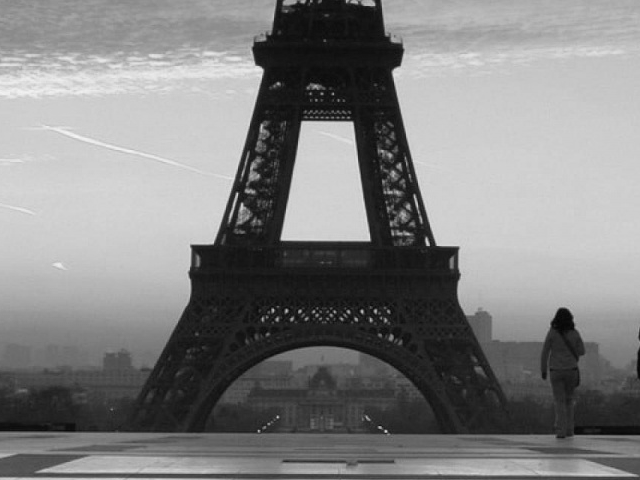
\includegraphics[height=0.4\textwidth]{fig/eiffel_grayscale}\\
\caption{Original Eiffel Tower grayscale image.}
\label{fig_eiffel_grayscale}
\end{center}
\end{figure}

\begin{figure}[ht!]
\begin{center}
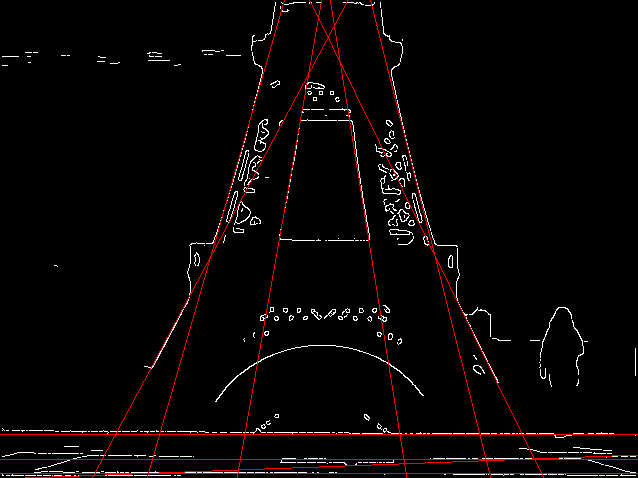
\includegraphics[height=0.4\textwidth]{fig/eiffel_hough}\\
\caption{Eiffel Tower image processed using the Hough Transform.}
\label{fig_eiffel_hough}
\end{center}
\end{figure}

\begin{figure}[ht!]
\begin{center}
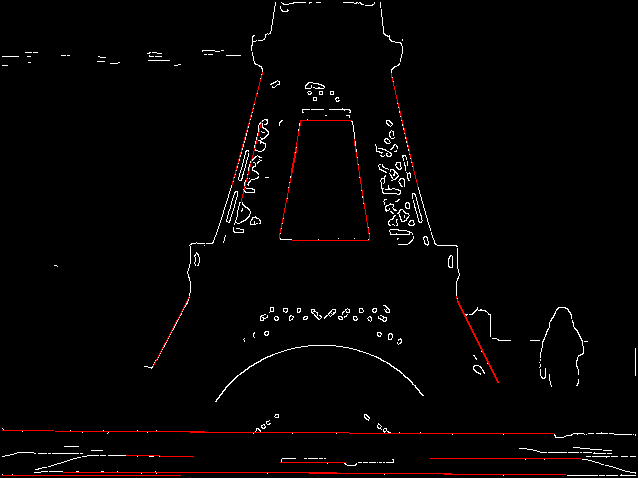
\includegraphics[height=0.4\textwidth]{fig/eiffel_phough}\\
\caption{Eiffel Tower image processed using the Probabilistic Hough Transform.}
\label{fig_eiffel_phough}
\end{center}
\end{figure}


\begin{itemize}
	\item Conceptual variant of the Hough Transform that solves its most important disadvantage.
	\item OpenCV has both implementations: Hough Transform and Probabilistic Hough Transform (most used).
\end{itemize}

\begin{table}
\begin{center}
\begin{tabular}{| l | c | c |}
\hline
\multicolumn{1}{|c|}{Parameter}	 & 	\multicolumn{1}{c|}{Traditional}	 & 	\multicolumn{1}{c|}{Probabilistic}\\ \hline
Total time (s)	& 	163.97	 &	154.52\\ \hline
Time per frame (ms)	& 	20.5	 & 	19.32\\ \hline
Frequency (Hz)		& 	48.79	 & 	51.77\\ \hline
\end{tabular}
\caption[Comparison of Hough transform algorithms.]{Comparison of Hough transform algorithms processing the same image 8000 times.}
\label{tab_compeiffel}
\end{center}
\end{table}


Both implementations were used to process the same image (Fig.~\ref{fig_eiffel_grayscale}) to compare their performance. The graphical result of the traditional algorithm is shown in figure \ref{fig_eiffel_hough}. The output of using the probabilistic variation is shown in figure \ref{fig_eiffel_phough}. Both algorithms were executed eight thousand times on the original images to avoid noise from unrelated software running during the experiment.

The following observations can be from the results:

\begin{itemize}
	\item The traditional algorithm does not compute lines' delimiting points (this is the reason lines cross through all the image).
	\item The probabilistic version detected all (and even more) the lines detected by its counterpart.
	\item A comparison of the time taken by both algorithms is shown in \ref{tab_compeiffel}.
	\item The ammount of time taken by the Probabilistic Hough Transform is slightly lower but it does more than the traditional one. It does much more in slightly less time.
	\item The line extraction parameters of the traditional algorithm are tuned and proved.
	\item Probabilistic Hough Transform parameters can still be tuned to get better results.
\end{itemize}

%%%%%%%%%%%%%%%%%%%%%%%%%%%%%%%%%%%%%%%%%%%%%%%%%%%%%%%%%%%%%%%%%%%%%%

\subsubsection{Planning}
Objectives were classified in the following categories:
\begin{itemize}
	\item \textbf{STM32:} Image acquisition and sending code.
	\item \textbf{Mechanic:} Hardware, mounting the cameras on the vehicle, etcetera.
	\item \textbf{Raspberry:} Image reception code and task management (pririties, scheduler, etcetera).
	\item \textbf{Vision:} Image processing.
	\item \textbf{Control:} Model extraction, control synthesis.
	\item \textbf{Paper:} Researching, documenting and publishing project results.
\end{itemize}

\subsection{Results}

%%%%%%%%%%%%%%%%%%%%%%%%%%%%%%%%%%%%%%%%%%%%%%%%%%%%%%%%%%%%%%%%%%%%%%

\subsubsection[Revisión bibliográfica transformada de Hough.]{Revisión bibliográfica de aplicaciones de la transformada de Hough.}
\begin{itemize}
	\item Se detectaron las principales debilidades de la transformada de Hough.
	\item Se vieron varias soluciones que se han propuesto para eficientizar la implementación.
	\item Se decidió implementar el código en C para la Transformada Probabilística de Hough.
\end{itemize}

%%%%%%%%%%%%%%%%%%%%%%%%%%%%%%%%%%%%%%%%%%%%%%%%%%%%%%%%%%%%%%%%%%%%%%

\subsubsection[Código C de la T. Probabilística de Hough]{Implementación en C de la Transformada Probabilística de Hough.}
\begin{itemize}
	\item Se implementó satisfacoriamente.
	\item Es una variación del concepto original que hace más en menos tiempo.
	\item Sigue hacer más optimizaciones al código y generalizarla para detectar vehículos.
\end{itemize}

%%%%%%%%%%%%%%%%%%%%%%%%%%%%%%%%%%%%%%%%%%%%%%%%%%%%%%%%%%%%%%%%%%%%%%

\subsubsection{Exploración de proyectos de STM32.}
\begin{itemize}
	\item Se recolectaron programas de ejemplo de las funciones que se usarán (DCMI, DMA, SPI).
	\item Está planeado empezar a compilar estos proyectos la próxima semana.
\end{itemize}

%%%%%%%%%%%%%%%%%%%%%%%%%%%%%%%%%%%%%%%%%%%%%%%%%%%%%%%%%%%%%%%%%%%%%%

\subsubsection{Planeación.}
\begin{itemize}
	\item Se definieron actividades a realizar para el objetivo.
	\item Se asignó una cantidad de tiempo aproximadoa a cada actividad en forma de Gantt (Fig.~{\ref{fig_ganttA}}).
\end{itemize}

\subsection{Pending}

\begin{itemize}
	\item \textbf{Camera mount structure design:} It was expected to be done this week, but it has been rescheduled to next week (Fig.~\ref{fig_ganttA}).
	\item \textbf{Purchase:} The components were expected for this week but they did not arrive.
	\item \textbf{Benchmarking/profiling:} A date was assigned to this task too. 
\end{itemize}

\clearpage

%%%%%%%%%%%%%%%%%%%%%%%%%%%%%%%%%%%%%%%%%%%%%%%

\fromto{May 12 - May 16}
\section{MEMORANDUM 03}

\subsection{Activities}

%%%%%%%%%%%%%%%%%%%%%%%%%%%%%%%%%%%%%%%%%%%%%%%%%%%%%%%%%%%%%%%%%%%%%%

\subsubsection{Camera mount design}
\begin{itemize}
	\item The electronic components were received this Monday.
	\item Measurements of the size of the camera and its PCB components were taken.
	\item After observing Carrita's front structure the only readily available mounting point was identified as a thin plate with four screw holes.
	\item Measurements of this thin plate were taken.
	\item A camera mount was designed aiming at:
	\begin{itemize}
		\item Centered cameras.
		\item Aligned cameras.
		\item Fixed, constant distance between cameras.
		\item Keeping a DOF (angle/inclination of view towards the floor).
	\end{itemize}
	\item CAD software was used to draft mechanisms and spot possible conflicts.
	\item After solving some design conflicts found the original concept part and drawings files were generated.
\end{itemize}


%%%%%%%%%%%%%%%%%%%%%%%%%%%%%%%%%%%%%%%%%%%%%%%%%%%%%%%%%%%%%%%%%%%%%%

\subsubsection{Edge detection research}
As mentioned in previous sections, the code used used for edge detection is from FAST-EDGE project. Some modifications were done to the arguments of the functions, the file loading code was removed and the functions were used to work directly on memory.

The code does mainly two things:
\begin{itemize}
	\item Gaussian blurs the image.
	\item Detectes and draws edges (white) over a black background.
\end{itemize}

These two processes' input and output were well known by me but their internals were not. I studied these topics to know which optimizations could be done to the code and which lacking functionality could be added.

The following conclussions can be made after studying the code and the theory behind it:
\begin{itemize}
	\item Region of interest (ROI) can be added to the code to avoid running the function on the whole image if it is not necessary.
	\item Functions are not inlined. This does not guarantee the compiler is not inlining but it is a potential boost.
	\item Fixed-point arithmetic is not used either.
\end{itemize}

The most useful and interesting finding of this research was that the code looked like it could be implemented on a GPU. This topic is presented in the next section.

%%%%%%%%%%%%%%%%%%%%%%%%%%%%%%%%%%%%%%%%%%%%%%%%%%%%%%%%%%%%%%%%%%%%%%

\subsubsection{General-purpose computing on graphics processing units}

Graphical processing units are highly parallelized processors used (mostly) for graphics. Central processing units may have multiple cores but they are far of being as powerful as a GPU when it comes to solving computations which can be parallelized. While reading the code behind edge detection I remembered GPGPU, which is using the GPU for computations typically done by a CPU (i.e. not graphics). 

Some GPU vendors have introduced or are introducing interfaces to freely use the GPU. The main open project for this is called OpenCL. For processors without OpenCL support, GPGPU computation has been done using OpenGL shaders to perform graphics-unrelated computations by mapping them to a graphics space (performing calculations of fast fourier transform and other digital signal processing operations much faster than on the host CPU).

Some (the most important) research results for related GPU published work are:
\begin{itemize}
	\item OpenCL is not supported on the Raspberry Pi.
	\item Raspberry Pi's OpenGL implementation is a complete OpenGL ES 2.0.
	\item This is a video\cite{cummings} showing Pi’s GPU computing and displaying sixteen textures.
	\begin{itemize}
		\item One of them is a Gaussian filter.
		\item All are drawn at the same time in real time.
		\item Output is sent out through HDMI 1080p.
		\item OpenGLSL code is available.
	\end{itemize}
	\item Markéta Dubská et al.\cite{dubska} show a GPU implementation of line detection using OpenGLSL.
	\begin{itemize}
		\item The GPU implementation outperforms OpenCV running on all the cores of an i7-920 processor.
		\item Code not available.
	\end{itemize}
	\item I have experience using OpenGL for graphics but not for computations.
	\item I began to study OpenGLSL because its an area worth of exploration.
	\begin{itemize}
		\item It has space for research and inovation.
		\item Impact on any device with an OpenGL ES 2.0 capable video card.
		\item This includes most smartphones
		\item Previous experience with OpenGL makes spending time on this less costly.
		\item On full success this will boost our possibilities significantly.
		\item Otherwise it will still help a bit.
	\end{itemize}
\end{itemize}

%%%%%%%%%%%%%%%%%%%%%%%%%%%%%%%%%%%%%%%%%%%%%%%%%%%%%%%%%%%%%%%%%%%%%%

\subsubsection{STM32 - IDE installation}

\begin{itemize}
	\item IDE options exploration.
	\item Two were installed and tested on Windows based on internet resources.
	\begin{itemize}
		\item CrossWorks for ARM.
		\item IAR Embedded Workbench ARM v7.10.
	\end{itemize}
	\item IAR Embedded Workbench will be used for the project because ST provides ready to use projects for it.
\end{itemize}

%%%%%%%%%%%%%%%%%%%%%%%%%%%%%%%%%%%%%%%%%%%%%%%%%%%%%%%%%%%%%%%%%%%%%%

\subsubsection{STM32 - SPI and DMA}
\begin{itemize}
	\item A communication test with the Raspberry Pi was performed, confirming the following keypoints work:
	\begin{itemize}
		\item IDE.
		\item Programmer.
		\item Debugger.
		\item SPI (slave mode) and DMA (memory to peripheral).
	\end{itemize}
\end{itemize}


%%%%%%%%%%%%%%%%%%%%%%%%%%%%%%%%%%%%%%%%%%%%%%%%%%%%%%%%%%%%%%%%%%%%%%

\subsubsection{Raspberry Pi - SPI}

The most common (and documented) way of accessing the SPI peripheral on the Raspberry Pi is through the Linux kernel module (whether accessed from python, shell, C). I knew it was not the fastest option but I did not know how the fastest one work. After the corresponding research and tests it can be noted that:

\begin{itemize}
	\item Kernel's SPI module does not allow "full freedom" access to the chip peripheral.
	\item This limits the transfer speed.
	\item bcm2835 library allows low-level access using high-level programming.
	\item The library was compiled and installed.
	\item A communication test with the STM32 was successfully done.
\end{itemize}

%%%%%%%%%%%%%%%%%%%%%%%%%%%%%%%%%%%%%%%%%%%%%%%%%%%%%%%%%%%%%%%%%%%%%%

\subsubsection{Raspberry Pi - Performance improvements}

\begin{itemize}
\item \textbf{GPU.} Already explained at another section. 
\item \textbf{Bare bones.} After finding the Linux is not needed for SPI usage the question about whether it was needed for anything arose and it turned out to be possible to run ARM code directly from the SD card. Work has been done on that. This is just something to have in mind because there are some very useful Linux features that are still needed (drivers, process management, pipelines).
\item \textbf{Overclocking.} An official maximum overclock was performed, this sets the Raspberry Pi clock at 1 GHz (42\% faster than without overclock).
\item \textbf{Shutdown unused modules.} Some Linux modules can be turned off to save CPU usage. That was known but an interesting finding was that the HDMI output can be turned off (which is a relatively heavy process that will not be needed). This is something to have in mind: turning down as many things as possible.
\end{itemize}

\subsection{Results}

%%%%%%%%%%%%%%%%%%%%%%%%%%%%%%%%%%%%%%%%%%%%%%%%%%%%%%%%%%%%%%%%%%%%%%

\subsubsection{Camera mount design}

\begin{itemize}
	\item Requirements definition.
	\item CAD part and drawing design. See figures \ref{fig_cammountp1}, \ref{fig_cammountp2} and \ref{fig_cammountp3} at the Appendix.
	\item Research on the camera's positioning for propper stere visions.
\end{itemize}

%%%%%%%%%%%%%%%%%%%%%%%%%%%%%%%%%%%%%%%%%%%%%%%%%%%%%%%%%%%%%%%%%%%%%%

\subsubsection{Edge detection research}

\begin{itemize}
	\item Knowledge about gaussian, sobel and canny theory used for edge detection.
	\item Possible optimizations to and limitations of the code were identified.
	\item Hint about GPU usage.
\end{itemize}

%%%%%%%%%%%%%%%%%%%%%%%%%%%%%%%%%%%%%%%%%%%%%%%%%%%%%%%%%%%%%%%%%%%%%%

\subsubsection{General-purpose computing on graphics processing units}

\begin{itemize}
	\item Knowledge about Pi's GPU.
	\item Pointers to GPU based solutions for the application.
	\item Study of OpenGLSL was started but not finished.
\end{itemize}

%%%%%%%%%%%%%%%%%%%%%%%%%%%%%%%%%%%%%%%%%%%%%%%%%%%%%%%%%%%%%%%%%%%%%%

\subsubsection{STM32 - IDE installation}

\begin{itemize}
	\item IAR Embedded Workbench ARM v7.10 was chosen and installed.
\end{itemize}

%%%%%%%%%%%%%%%%%%%%%%%%%%%%%%%%%%%%%%%%%%%%%%%%%%%%%%%%%%%%%%%%%%%%%%

\subsubsection{STM32 - SPI and DMA}
\begin{itemize}
	\item Successful communication test in slave mode (using DMA) with the Raspberry Pi.
\end{itemize}

%%%%%%%%%%%%%%%%%%%%%%%%%%%%%%%%%%%%%%%%%%%%%%%%%%%%%%%%%%%%%%%%%%%%%%

\subsubsection{Raspberry Pi - SPI}

\begin{itemize}
	\item Low level library installed. This allows using SPI directly commanding the processor (skipping the Linux kernel).
	\item Successful communication test in master mode with the STM32 as slave.
\end{itemize}

%%%%%%%%%%%%%%%%%%%%%%%%%%%%%%%%%%%%%%%%%%%%%%%%%%%%%%%%%%%%%%%%%%%%%%

\subsubsection{Raspberry Pi - Performance improvements}

\begin{itemize}
	\item A prioritized list (for the application at hand) of potential optimizations to have in mind:
	\begin{itemize}
		\item Using the GPU for image processing.
		\item Overclocking.
		\item Shutdown unused modules.
		\item Running the raspberry "bare bones", without Linux.
	\end{itemize}
\end{itemize}

\subsection{Pending}

\begin{itemize}
	\item \textbf{Manufacture of the camera mount mechanism:} The mechanism was not manufactured but it was decided that a simpler one will be used to see the effect of vibrations on line detection in general before building the final one.
	\item \textbf{DCMI test:} I spent some time turning the LCD off (because it conflicts with the DCMI pins) and deciding which of the board pins are the best to use. This had a software-side learning curve.
	\item \textbf{Region of interest:} The time that was planned to be used on implementing ROI to the vision algorithms was spent studying OpenGLSL because the implementation of ROI will be different on the GPU.
\end{itemize}

\clearpage

%%%%%%%%%%%%%%%%%%%%%%%%%%%%%%%%%%%%%%%%%%%%%%%

\fromto{May 19 - May 23}
\section{MEMORANDUM 04}

\subsection{Activities}

%%%%%%%%%%%%%%%%%%%%%%%%%%%%%%%%%%%%%%%%%%%%%%%%%%%%%%%%%%%%%%%%%%%%%%

\subsubsection{Raspberry Pi - Install new vision dependencies}
\begin{itemize}
	\item Dependencies to run vision code were installed to the raspberry.
	\item Line detection CPU code was compiled and run.
	\item Optimizations are still needed but frame-reading from the cameras must be completed first to know which are the best options.
\end{itemize}

%%%%%%%%%%%%%%%%%%%%%%%%%%%%%%%%%%%%%%%%%%%%%%%%%%%%%%%%%%%%%%%%%%%%%%

\subsubsection{Raspberry Pi - SPI reception of images}
\begin{itemize}
	\item Code was started to receive and manage the data from the STM32.
	\item Maximum possible transfer speed was experimentally found to be around 43 MHz.
	\begin{itemize}
		\item STM32 datasheet states its maximum SPI transfer speed is 45 Mbits/s.
		\item Raspberry Pi can transfer up to 125 Mbits/s.
		\item The next Pi "step" goes beyond STM32 transfer limit and fails.
	\end{itemize}
	\item This is scheduled (Gantt) to be finished next week.
\end{itemize}

%%%%%%%%%%%%%%%%%%%%%%%%%%%%%%%%%%%%%%%%%%%%%%%%%%%%%%%%%%%%%%%%%%%%%%

\subsubsection{STM32 - DCMI}
\begin{itemize}
	\item DCMI controller was programmed and used successfully.
	\item Pin options were found to avoid conflicts with wired but not used peripherals and with the required ones (see next section).
	\item This was a crucial part of the development because it allows to get frames off the camera using only hardware.
\end{itemize}

%%%%%%%%%%%%%%%%%%%%%%%%%%%%%%%%%%%%%%%%%%%%%%%%%%%%%%%%%%%%%%%%%%%%%%

\subsubsection{STM32 - Pin selection}
\begin{itemize}
	\item The 32F429IDISCOVERY board has some peripherals soldered to pins used by the DCMI controller and the high speed SPI peripherals.
	\item These conflicts had to be addressed to be able to safely use these required features.
	\item The microcontroller has options for many of the required DCMI signals.
	\begin{itemize}
		\item Table \ref{tab_boardpin_dcmi} shows the DCMI signals of interest and the pins they could be mapped to.
		\item The board column shows the peripheral the corresponding pin is soldered to at the discovery board.
		\item It can be seen there are no free options for every signal, thus the LCD peripheral can not be used simultaneously. 
	\end{itemize}
\end{itemize}
\begin{table}[ht!]
\begin{center}
\begin{tabular}{| c | c | c | c | c | c | c |}
\hline
\multicolumn{1}{|c|}{DCMI}	 & 	\multicolumn{1}{c|}{Pin}	 & 	\multicolumn{1}{c|}{Board} & 	\multicolumn{1}{c|}{Pin}	 & 	\multicolumn{1}{c|}{Board} & 	\multicolumn{1}{c|}{Pin}	 & 	\multicolumn{1}{c|}{Board}\\ \hline
D0	&	PA9	&	Free	&	PC6	&	\scriptsize LCD-TFT \& LCD-RGB	&		&	\\
D1	&	PA10	&	Free	&	PC7	&	\scriptsize LCD-TFT \& LCD-RGB	&		&	\\
D2	&	PC8	&	Free	&	PG10	&	\scriptsize LCD-TFT \& LCD-RGB	&	PE0	&	SDRAM\\
D3	&	PG11	&	\scriptsize LCD-TFT \& LCD-RGB	&	PC9	&	\scriptsize ACP/RF \& Touch panel	&	PE1	&	SDRAM\\
D4	&	PE4	&	Free	&	PC11	&	Free	&		&	\\
D5	&	PD3	&	\scriptsize LCD-TFT \& LCD-RGB	&	PB6	&	SDRAM	&		&	\\
D6	&	PE5	&	Free	&		&		&		&	\\
D7	&	PE6	&	Free	&	PB9	&	\scriptsize LCD-TFT \& LCD-RGB	&		&	\\
HSYNC	&	PA4	&	\scriptsize LCD-TFT \& LCD-RGB	&		&		&		&	\\
VSYNC	&	PB7	&	Free	&	PG9	&	Free	&		&	\\
PXCLK	&	PA6	&	\scriptsize LCD-TFT \& LCD-RGB	&		&		&		&	\\ \hline
\end{tabular}
\caption[Pin options for each DCMI signal.]{Pin options for each DCMI signal according to the microcontroller's datasheet and the peripheral they are connected to at the discovery board.}
\label{tab_boardpin_dcmi}
\end{center}
\end{table}

\begin{itemize}
	\item Table \ref{tab_boardpin_dcmi_conflict} shows the signal the chosen conflicted pins carry.
	\begin{itemize}
		\item It can be seen that there is an input pin and some inputs/outputs ones.
		\item The only LCD datasheet available is very poor.
		\item It does not explicitly state what happens with those pins if you disable the screen (using its EN input).
		\item It does not states in which circumstances the DX pins behave as outputs.
		\item These lines behave as inputs when running the LCD example code.
		\item The LCD was disabled and no situation was found for any of these pins behaving as outputs.
	\end{itemize}

\end{itemize}

\begin{table}[ht!]
\begin{center}
\begin{tabular}{| c | c | c | c | c |}
\hline
\multicolumn{1}{|c|}{Conflicted pin}	 & 	\multicolumn{1}{c|}{LCD TFT}	 & 	\multicolumn{1}{c|}{LCD RGB} & 	\multicolumn{1}{c|}{I/O}	 & 	\multicolumn{1}{c|}{Action}\\ \hline
PA4	&	VSYNC	&	VSYNC	&	I	&	Nothing\\
PA6	&	DB6	&	G2	&	I/O	&	Force input or float\\
PD3	&	DB11	&	G7	&	I/O	&	Force input or float\\
PG11	&	DB11	&	B3	&	I/O	&	Force input or float\\ \hline
\end{tabular}
\caption[Discovery board DCMI non-free pins.]{Discovery board DCMI non-free pins and the action to trigger at the target device to avoid problems.}
\label{tab_boardpin_dcmi_conflict}
\end{center}
\end{table}


\begin{itemize}
	\item High speed SPI peripheral were also:
	\begin{itemize}
		\item already soldered to something or
		\item their pins were used by the DCMI controller.
	\end{itemize}
	\item High speed SPI instances are SPI1, SPI 4 (table \ref{tab_boardpin_spi_a}), SPI5 and SPI6 (table \ref{tab_boardpin_spi_b}).
	\item Conflicts can be seen on these tables.
	\item The only option that does not conflict with SDRAM nor DCMI is SPI5.
\end{itemize}


\begin{table}[ht!]
\begin{center}
\begin{tabular}{| c | c | c | c | c |}
\hline
\multirow{2}{*}{Signal}	&	\multicolumn{2}{|c|}{SPI1}		&	\multicolumn{2}{|c|}{SPI4}\\ \cline{2-5}
	&	Posible Pin	&	Datasheet	&	Posible Pin	&	Datasheet	\\ \hline
\multirow{2}{*}{SCK}	&	PA5	&	Free	&	PE12	&	SDRAM	\\
	&	PB3	&	System	&	PE2	&	Free	\\ \hline
\multirow{2}{*}{MOSI}	&	PB5	&	SDRAM	&	PE6	&	Free	\\
	&	PA7	&	ACP/RF	&	PE14	&	SDRAM	\\ \hline
\multirow{2}{*}{MISO}	&	PB4	&	Free	&	PE5	&	Free	\\
	&	PA6	&	LCD-TFT \& LCD-RGB	&	PE13	&	SDRAM	\\ \hline
\multirow{2}{*}{NSS}	&	PA15	&	Touch panel	&	PE11	&	SDRAM \\
	&	PA4	&	LCD-TFT \& LCD-RGB	&	PE4	&	Free \\ \hline
\end{tabular}
\caption[Options for each SPI signal (SPI1 and SPI2).]{Options for each SPI signal (SPI1 and SPI2) according to microcontroller's datasheet and the peripheral they are connected to on the discovery board.}
\label{tab_boardpin_spi_a}
\end{center}
\end{table}

\begin{table}[ht!]
\begin{center}
\begin{tabular}{| c | c | c | c | c | c | c | c | c |}
\hline
\multirow{2}{*}{Signal}	&	\multicolumn{2}{|c|}{SPI5}		&	\multicolumn{2}{|c|}{SPI6}	\\ \cline{2-5}
	&	Posible Pin	&	Datasheet	&	Posible Pin	&	Datasheet \\ \hline
SCK	&	PF7	&	\scriptsize LCD-TFT \& LCD-SPI \& L3GD20	&	PG13	&	LED \\ \hline
\multirow{2}{*}{MOSI}	&	PF9	&	\scriptsize LCD-TFT \& LCD-SPI \& L3GD20	&	PG14	&	LED \\
	&	PF11	&	SDRAM	&		&	\\ \hline
MISO	&	PF8	&	L3GD20	&	PG12	&	\scriptsize LCD-TFT \& LCD-RGB \\ \hline
NSS	&	PF6	&	Free	&	PG8	&	SDRAM \\ \hline
\end{tabular}
\caption[Options for each SPI signal (SPI5 and SPI6).]{Options for each SPI signal (SPI5 and SPI6) according to microcontroller's datasheet and the peripheral they are connected to on the discovery board.}
\label{tab_boardpin_spi_b}
\end{center}
\end{table}


\begin{itemize}
	\item SPI was easier to address because it is actually a SPI feature to allow connection of multiple slaves. 
	\item The only action taken to ensure there were no conflicts was to pull the chip/slave select signal of the two connected peripherals (table \ref{tab_boardpin_spi5_conflict}) up.
\end{itemize}

\begin{table}[ht!]
\begin{center}
\begin{tabular}{| c | c | c | c | c |}
\hline
Conflicted pin	&	LCD TFT	&	LCD RGB	&	L3GD20 \\ \hline
PF7	&	DCX	&	SCL	&	SCK \\
PF8	&	-	&	-	&	MISO \\
PF9	&	SDA	&	SDI/SDO	&	MOSI \\ \hline
\end{tabular}
\caption[Discovery board SPI5 non-free pins.]{Discovery board SPI5 non-free pins and the signal they carry. It is only necessary to keep the SS pins high for these devices.}
\label{tab_boardpin_spi5_conflict}
\end{center}
\end{table}


\begin{itemize}
	\item All the pins involved with the interfacing of the camera and the Raspberry are shown at table \ref{tab_boardpin_final}. 
	\item MCO is the peripheral used to generate clock signals out of the microcontroller oscillators
	\begin{itemize}
		\item It is used as the camera's clock signal.
	\end{itemize}
\end{itemize}
\begin{table}[ht!]
\begin{center}
\begin{tabular}{| c | c | c |}
\hline
Pin	&	Peripheral	&	Signal\\ \hline
PA04	&	\multirow{11}{*}{DCMI}	&	HSYNC\\
PA06	&		&	PXCLK\\
PA09	&		&	D0\\
PA10	&		&	D1\\
PB07	&		&	VSYNC\\
PC08	&		&	D2\\
PD03	&		&	D5\\
PE04	&		&	D4\\
PE05	&		&	D6\\
PE06	&		&	D7\\
PG11	&		&	D3\\ \hline
PC01	&	\multirow{7}{*}{GPIO}	&	CS Gyro\\
PC02	&		&	CS LCD\\
PF10	&		&	EN LCD\\ 
PC11	&		&	SDIOC\\
PC12	&		&	SDIOD\\
PD04	&		&	REQ\\
PD05	&		&	RDY\\ \hline
PC09	&	MCO	&	MCO2\\ \hline
PF07	&	\multirow{2}{*}{SPI5}	&	SCK\\
PF08	&		&	MISO\\ \hline
\end{tabular}
\caption[Final selections of pins.]{Final selections of pins to be used by the application.}
\label{tab_boardpin_final}
\end{center}
\end{table}


%%%%%%%%%%%%%%%%%%%%%%%%%%%%%%%%%%%%%%%%%%%%%%%%%%%%%%%%%%%%%%%%%%%%%%

\subsubsection{General-purpose computing on graphics processing units}
\begin{itemize}
	\item Finished study of OpenGL ES 2.0 features of interest.
	\item A very interesting point is that WebGL (OpenGL implementation included in most moder web browsers) is based on OpenGL ES 2.0.
	\item This was used to validate earned knowledge knowing code would be easily ported to the Raspberry Pi.
	\item GPU code for Gauss and Sobel filters was developed and tested.
	\item Limitations were found but there is no way to meassure their impact without having the frame reception code ready.
\end{itemize}


\subsection{Results}

\subsubsection{Raspberry Pi - Install new vision dependencies}
\begin{itemize}
	\item All the required software was installed and tested on the Pi.
	\item Further work needs frame reception code to be finished first.
\end{itemize}

\subsubsection{Raspberry Pi - SPI reception of images}
\begin{itemize}
	\item Previous SPI test were done by sending a string.
	\item Code for receiving and managing images at STM32's maximum speed was started.
\end{itemize}

\subsubsection{STM32 - DCMI}
\begin{itemize}
	\item Successfully used STM32's DCMI controller to manage camera output through hardware.
\end{itemize}

\subsubsection{STM32 - Pin selection}
\begin{itemize}
	\item All the required signals were assigned to a pin of the discovery board.
	\item Conflicts with wired peripherals were solved.
\end{itemize}

\subsubsection{General-purpose computing on graphics processing units}
\begin{itemize}
	\item Finished study of OpenGL ES 2.0 features of interest.
	\item Reached a point where answers must be found by experimentation (due to the lack of documentation).
	\item Further work needs frame reception code to be finished first.
\end{itemize}

\subsection{Pending}

\begin{itemize}
	\item \textbf{Use of SDRAM:} The external STM32's memory soldered to the discovery board has not been used in any test.
	\item \textbf{Frame transfer to the Raspberry:} This became a bottleneck. Finalization of this task is scheduled for the next week but some final tests deppend on this.
\end{itemize}

\clearpage

%%%%%%%%%%%%%%%%%%%%%%%%%%%%%%%%%%%%%%%%%%%%%%%

\fromto{May 26 - May 30}
\section{MEMORANDUM 05}

\subsection{Activities}

%%%%%%%%%%%%%%%%%%%%%%%%%%%%%%%%%%%%%%%%%%%%%%%%%%%%%%%%%%%%%%%%%%%%%%

\subsubsection{DCMI troubleshooting}
\begin{itemize}
	\item When trying to send images to the Raspberry using DMA it was found most data were zeros.
	\item A lot of different software and hardware tests were done to diagnose the problem.
	\begin{itemize}
		\item DCMI interrupts work as expected.
		\item DMA works.
		\item If you disconnect a data pin DMA writes a one (due to STM32's pull-up resistor).
		\item Every signal looks as expected using an oscilloscope.
	\end{itemize}
	\item It seems to be a hardware problem but what does not make sense is that you can (slowly) capture the camera data using software (without DCMI).
\end{itemize}

%%%%%%%%%%%%%%%%%%%%%%%%%%%%%%%%%%%%%%%%%%%%%%%%%%%%%%%%%%%%%%%%%%%%%%


\subsection{Results}

\subsubsection{DCMI troubleshooting}
\begin{itemize}
	\item I was not able to get data out of the camera using DCMI.
	\item This is very strange because different tests discard possible problems.
\end{itemize}

\subsection{Pending}

\begin{itemize}
	\item \textbf{Integration:} Everything was delayed due to inability to get DCMI to work.
\end{itemize}

\clearpage

%%%%%%%%%%%%%%%%%%%%%%%%%%%%%%%%%%%%%%%%%%%%%%%

\fromto{Jun 02 - Jun 06}
\section{MEMORANDUM 06}

\subsection{Activities}

%%%%%%%%%%%%%%%%%%%%%%%%%%%%%%%%%%%%%%%%%%%%%%%%%%%%%%%%%%%%%%%%%%%%%%

\subsubsection{OV7670 deep exploration}
\begin{itemize}
	\item While trying to find the cause of the DCMI problem the OV7670 chip was studied.
	\item Code to read and write to its internal registers was ported.
	\item Different registers configurations were attempted and used to try to make it easier for the software implementation to sample the data.
	\item Linux drivers' register sets were attempted without any good results.
\end{itemize}


%%%%%%%%%%%%%%%%%%%%%%%%%%%%%%%%%%%%%%%%%%%%%%%%%%%%%%%%%%%%%%%%%%%%%%

\subsubsection{DCMI software workaroud}
\begin{itemize}
	\item After trying some new ideas and doing more tests it was decided to attempt to read the camera in software.
	\item The objective was to:
	\begin{itemize}
		\item Read and interpret VSYNC, HREF and PXCLK signals.
		\item Read data lines (D0-D7) at the rising edge of the PXCLK signal if HREF is high and VSYNC is low.
	\end{itemize}
	\item The main problems found while doing this were:
	\begin{itemize}
		\item Compiler's optimizations impact results greatly (deleting an unrelated variable would make a difference between the program succeeding/failing).
		\item Impossibility to keep up with the data rate (sampling 8 lines of data in a very short ammount of time).
	\end{itemize}
	\item Pins were reassigned to be on the same port to make it possible to sample all the data with a single volatile read.
	\item Software branches were minimized supported by the new pin assignment and OV7670's register configurations (i.e. there is a mode that makes the PXCLK toggle only if HREF is active).
	\item This allowed to get a low resolution image at 30 fps.
	\item However the image was very noisy.
\end{itemize}

%%%%%%%%%%%%%%%%%%%%%%%%%%%%%%%%%%%%%%%%%%%%%%%%%%%%%%%%%%%%%%%%%%%%%%

\subsubsection{Integration with the Raspberry}
\begin{itemize}
	\item Integration was done using the code to read the image in software.
	\item A simple acknowledgment method is used.
	\begin{itemize}
		\item Two lines were connected between the Raspberry and the STM32.
		\item One is !REQUEST (active-low, Raspberry output, STM32 input) and the other one is !READY (active-low, STM32 output, Raspberry input).
		\item When the raspberry wants the next camera's frame it clears the !REQUEST line.
		\item When the STM32 has finished reading a complete frame it clears the !READY line.
		\item The frame is transferred through SPI.
		\item This needs to be done this way because Raspberry can not be the SPI slave.
		\item Double buffered mode can be implemented (interrupting the current frame capture and send the latest fully captured one) but was not because software "DCMI" is a temporal solution.
	\end{itemize}
	\item Integration and communication work.
	\item However, due to the very high image noise, vision algorithms were not even attempted.
\end{itemize}

%%%%%%%%%%%%%%%%%%%%%%%%%%%%%%%%%%%%%%%%%%%%%%%%%%%%%%%%%%%%%%%%%%%%%%

\subsection{Results}

%%%%%%%%%%%%%%%%%%%%%%%%%%%%%%%%%%%%%%%%%%%%%%%%%%%%%%%%%%%%%%%%%%%%%%

\subsubsection{OV7670 deep exploration}
\begin{itemize}
	\item Camera registers were explored.
	\item Code to read and write OV7670's registers was ported.
	\item Different configurations were attempted.
	\item Both from linux drivers and simple configurations.
\end{itemize}


%%%%%%%%%%%%%%%%%%%%%%%%%%%%%%%%%%%%%%%%%%%%%%%%%%%%%%%%%%%%%%%%%%%%%%

\subsubsection{DCMI software workaroud}
\begin{itemize}
	\item Software method was used to read frames out of the camera at low resolution, grayscale and 30 fps.
	\item The image was extremely noisy.
\end{itemize}

%%%%%%%%%%%%%%%%%%%%%%%%%%%%%%%%%%%%%%%%%%%%%%%%%%%%%%%%%%%%%%%%%%%%%%

\subsubsection{Integration with the Raspberry}
\begin{itemize}
	\item Integration was developed and tested.
	\item It works reliably.
\end{itemize}

%%%%%%%%%%%%%%%%%%%%%%%%%%%%%%%%%%%%%%%%%%%%%%%%%%%%%%%%%%%%%%%%%%%%%%

\subsection{Pending}

\begin{itemize}
	\item \textbf{Get the camera working properly:} Software "DCMI" works but only at low resolutions and the image is not really usable due to very high noise (but that seems to be a problem with the camera). This is the very last electronics step.
\end{itemize}

\clearpage

%%%%%%%%%%%%%%%%%%%%%%%%%%%%%%%%%%%%%%%%%%%%%%%%

\fromto{Jun 09 - Jun 13}
\section{MEMORANDUM 07}

\subsection{Activities}

%%%%%%%%%%%%%%%%%%%%%%%%%%%%%%%%%%%%%%%%%%%%%%%%%%%%%%%%%%%%%%%%%%%%%%

\subsubsection{Hardware image acquisition}
\begin{itemize}
	\item DMA and DCMI registers were modified directly (without using any library).
	\item Hardware image acquisition allows to get full framerate (30 fps) at full resolution (VGA) into memory.
	\item Final working setup is as follows:
	\begin{itemize}
		\item External crystal oscillator (8MHz) divided by two feeds the camera, which uses its PLL to get 24MHz. This resulted in better (less noise, more squared) signals.
		\item Pin configuration from table~\ref{tab_boardpin_final} was mantained.
		\item Code can be seen at the appendix.
	\end{itemize}
\end{itemize}

\subsubsection{OV7670 register configuration}
\begin{itemize}
	\item There are some values that need to be adjusted to get a good image. For example, with the default registers the image is very sensible to light: if you point it towards something white it blanks out any other non-white color.
	\item There are many register sets floating around the internet.
	\item Different register sets yield different results and may be written to easily change between register sets (recompilation is needed at the moment).
\end{itemize}

\subsubsection{STM32-Raspberry Pi communication protocol}

\begin{figure}[ht!]
\begin{center}
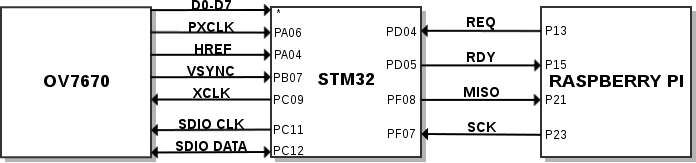
\includegraphics[height=0.22\textwidth]{fig/hwconnections}\\
\caption{Signals connected between the OV7670, the STM32 and the Raspberry Pi.}
\label{fig_hwconnections}
\end{center}
\end{figure}

\begin{itemize}
	\item Final hardware connections are shown in figure \ref{fig_hwconnections}.
	\begin{itemize}
		\item D0-D7 data lines were omitted but can be seen at table \ref{tab_boardpin_final}.
		\item Arrows indicate the data flow direction. The only bidirectional line is SDIO DATA.
		\item Transfers between the camera and the STM32 are handled by STM32's DCMI peripheral.
		\item Transfers between the STM32 and the Raspberry Pi are handled by their corresponding SPI peripherals.
		\item These are the minimal connections needed to get the image (from the OV7670) to the Raspberry Pi at a high datarate.
	\end{itemize}
\end{itemize}

\begin{figure}[ht!]
\begin{center}
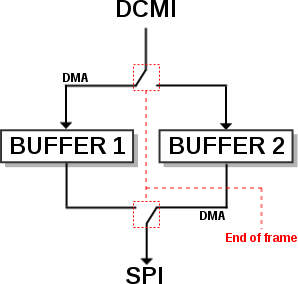
\includegraphics[height=0.45\textwidth]{fig/doublebuffer}\\
\caption{Double buffered DMA architecture. The end of frame toggles both pointers so the Raspberry always receives a full frame.}
\label{fig_doublebuffer}
\end{center}
\end{figure}

\begin{itemize}
	\item Double buffering was implemented.
	\begin{itemize}
		\item The SPI always points to the buffer the DCMI is not writing to.
		\item When a frame is completely captured, the buffers are toggled.
		\item This ensures only full and correct frames are sent to the Raspberry.
	\end{itemize}
\end{itemize}

\begin{figure}[ht!]
\begin{center}
\scalebox{1.5}{
\begin{tikztimingtable}
	REQ			& H L L 13{H} ;[dotted] 2{H}; 5{H} \\
	RDY			& H H 14{L} ;[dotted] 2{L}; 3{L} H H \\
	CLK			& L L L 13{C} ;[dotted] 2{C}; 3{C} L\\
	MISO			& U U U 18D{Image pixel data} U U\\
\end{tikztimingtable}
}
\caption{Time diagram showing the communication protocol between the Raspberry and the STM32.}
\label{fig_req_frame_time}
\end{center}
\end{figure}

\begin{itemize}
	\item A small request-response signaling needs to be performed before each transfer because the Raspberry Pi can not be the SPI slave (hardware limitation).
	\item This signaling's time diagram is shown in figure \ref{fig_req_frame_time}.
	\begin{itemize}
		\item Raspberry clears the REQ line, informing the STM32 it wants to start a SPI transfer.
		\item STM32 sets up the SPI buffer to the latest full frame and clears the RDY line.
		\item The Raspberry sets the REQ line and starts the SPI transfer.
		\item STM32 sets the RDY line when the transfer is complete.
	\end{itemize}
\end{itemize}

\subsubsection{Computer vision integration}
\begin{itemize}
	\item This task was started but there are still some things to adapt to fully run computer vision code on the received images.
\end{itemize}


%%%%%%%%%%%%%%%%%%%%%%%%%%%%%%%%%%%%%%%%%%%%%%%%%%%%%%%%%%%%%%%%%%%%%%


\subsection{Results}

\subsubsection{Hardware image acquisition}
Image acquisition by hardware (DCMI+DMA) has been implemented successfully after modifying every register directly (without using any library).

\subsubsection{OV7670 register configuration}
\begin{itemize}
	\item Some registers sets were loaded.
	\item The best register set for the situation (environment) should be loaded.
	\item Code may be written to chose between register sets at run time.
\end{itemize}

\subsubsection{STM32-Raspberry Pi communication protocol}
\begin{itemize}
	\item Some bugs at the communication protocol were fixed.
	\item Successful tests were done to send hardware acquired images.
\end{itemize}

\subsubsection{Computer vision integration}
\begin{itemize}
	\item This task was started but there are still some things to adapt to fully run computer vision code on the received images.
\end{itemize}

\subsection{Pending}

\begin{itemize}
	\item \textbf{Computer vision integration:} This will be done in the next days.
	\item \textbf{Optimize integrated system:} Tune the needed optimizations to get the highest frequency of data.
	\item \textbf{Mechanical camera mount.}
\end{itemize}

\clearpage

%%%%%%%%%%%%%%%%%%%%%%%%%%%%%%%%%%%%%%%%%%%%%%%%

\fromto{Jun 16 - Jun 20}
\section{MEMORANDUM 08}

\subsection{Activities}

\subsubsection{STM32 code improvements}
\begin{itemize}
	\item Now using the external SDRAM.
	\item ST's peripheral library did not allow continuous SPI transfers larger than 65535 bytes.
	\begin{itemize}
		\item This was not a problem on low resolutions.
		\item Larger resolutions segmentated a lot and this significantly increases transmission time.
		\item A combination of EXTI+DMA was implemented to allow single-stream SPI transfers of any size.
		\item This required some changes at the signaling protocol.
		\item All this is library-free code (directly modifying the microcontroller's registers).
	\end{itemize}
	\item Found out at the camera's datasheet that it can be overclocked on low resolutions.
	\item The new transmission signaling is shown in figure \ref{fig_start_frame_time}.
	\begin{itemize}
		\item The START and END signals are driven at the same time.
		\item This is because if only one ISR was written the microprocessor would loss the timing.
		\item STM32's EXTI does not differentiate between rising and falling edges if you want to detect both.
		\item Only one Raspberry signal is needed if it is connected to both STM32 pins.
	\end{itemize}
\end{itemize}
\begin{figure}[ht!]
\begin{center}
\scalebox{1.5}{
\begin{tikztimingtable}
	START			& H H 14{L} ;[dotted] 2{L}; 3{L} H H \\
	END			& H H 14{L} ;[dotted] 2{L}; 3{L} H H \\
	CLK			& L L L 13{C} ;[dotted] 2{C}; 3{C} L\\
	MISO			& U U U 18D{Image pixel data} U U\\
\end{tikztimingtable}
}
\caption{Time diagram showing the new communication protocol between the Raspberry and the STM32.}
\label{fig_start_frame_time}
\end{center}
\end{figure}

%%%%%%%%%%%%%%%%%%%%%%%%%%%%%%%%%%%%%%%%%%%%%%%%%%%%%%%%%%%%%%%%%%%%%%

\subsubsection{Computer vision integration}
\begin{itemize}
	\item The integration was finished.
	\item Current software on the Raspberry Pi side does the following:
	\begin{itemize}
		\item Allocates memory to store frames in every processing stage.
		\item Initializes the SPI peripheral.
		\item Signal the STM32 and read a frame from it.
		\item Optionally draws the frame at any processing stage (see figure \ref{fig_line_detection_integration}) using SDL.
		\item Performs Gaussian blurring, Edge detection and Probabilistic Hough Transform.
		\item Discriminates between lines and outputs the angle of the most important one through UART.
		\item All of the above using the laptop's camera (was needed for testing).
	\end{itemize}
\end{itemize}
\begin{figure}[ht!]
\begin{center}
\includegraphics[height=0.35\textwidth]{fig/line_detection_integration}\\
\caption{Steps of line detection running on the Raspberry.}
\label{fig_line_detection_integration}
\end{center}
\end{figure}


%%%%%%%%%%%%%%%%%%%%%%%%%%%%%%%%%%%%%%%%%%%%%%%%%%%%%%%%%%%%%%%%%%%%%%

\subsubsection{Stereo vision depth detection}
\begin{itemize}
	\item This opperation needs to be done on the GPU due to time constraints.
	\begin{itemize}
		\item It is a hevy operation and the CPU could not do it.
		\item An approximate solution needs to be calculated using the GPU.
	\end{itemize}
	\item Raspberry code was started to:
	\begin{itemize}
		\item Initialize, allocate and communicate with the GPU.
		\item Send the camera frames to the GPU.
		\item Perform custom operations on the frames using shaders.
		\item Draw the output.
	\end{itemize}
\end{itemize}

\subsection{Results}

\subsubsection{STM32 code improvements}
\begin{itemize}
	\item SDRAM is being used to store the frames.
	\item SPI code was modified to do SPI transfers of any size.
\end{itemize}

%%%%%%%%%%%%%%%%%%%%%%%%%%%%%%%%%%%%%%%%%%%%%%%%%%%%%%%%%%%%%%%%%%%%%%

\subsubsection{Computer vision integration}
\begin{itemize}
	\item Computer vision (for line detection) integration has been completed.
	\item Minor bugs need to be fixed.
	\item Optimizations are yet to be implemented
\end{itemize}

%%%%%%%%%%%%%%%%%%%%%%%%%%%%%%%%%%%%%%%%%%%%%%%%%%%%%%%%%%%%%%%%%%%%%%

\subsubsection{Stereo vision depth detection}
\begin{itemize}
	\item GPU is initialized propperly.
	\item Shadders are being executed on the framebuffers.
	\item Output is being drawn correctly.
	\item The camera->GPU connection is not done yet (constant data was being loaded to test all of the above).
\end{itemize}

\subsection{Pending}

\begin{itemize}
	\item \textbf{Turn line detection onto lane detection:} Add appropiate discrimination rules to get the lane.
	\item \textbf{GPU communication and shader programming:} Test shaders are working but the ones that give approximate solutions to the problem must be written, using the camera as the input is also yet to be written.
	\item \textbf{Mechanical camera mount.}
\end{itemize}

\clearpage

%%%%%%%%%%%%%%%%%%%%%%%%%%%%%%%%%%%%%%%%%%%%%%%%

\fromto{Jun 23 - Jun 27}
\section{MEMORANDUM 09}

\subsection{Activities}

%%%%%%%%%%%%%%%%%%%%%%%%%%%%%%%%%%%%%%%%%%%%%%%%%%%%%%%%%%%%%%%%%%%%%%

\subsubsection{Stereo vision depth detection}
\begin{itemize}
	\item Camera frames are read by the CPU.
	\item CPU writes the images to the GPU.
	\item Designed the rendering pipeline needed by our application.
	\item The pipeline generates the following framebuffers:
	\begin{itemize}
		\item \textbf{Encoding:} This is the same data than the original image, but using the RGBA channels to pack four GL\_LUMINANCE 	pixels into a GL\_RGBA pixel. See figure~\ref{fig_pixel_pack} for a graphical explanation.
		\item \textbf{Support window:} This puts in every pixel information about its surrounding pixels. The objective is to make the calculation of the disparity map computationally cheaper. See figure~\ref{fig_support_window} for a graphical explanation.
		\item \textbf{Disparity map:} This looks for the disparity where the similarity of the support windows is a minimum and generates a texture with this information.
	\end{itemize}
\end{itemize}

\begin{figure}[ht!]
\begin{center}
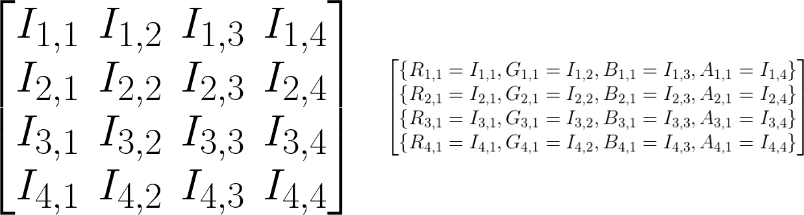
\includegraphics[height=0.22\textwidth]{fig/pixel_pack}\\
\caption{4x4 GL\_LUMINANCE texture (left) losslessly packed into a 4x1 GL\_RGBA texture (right).}
\label{fig_pixel_pack}
\end{center}
\end{figure}

\begin{figure}[ht!]
\begin{center}
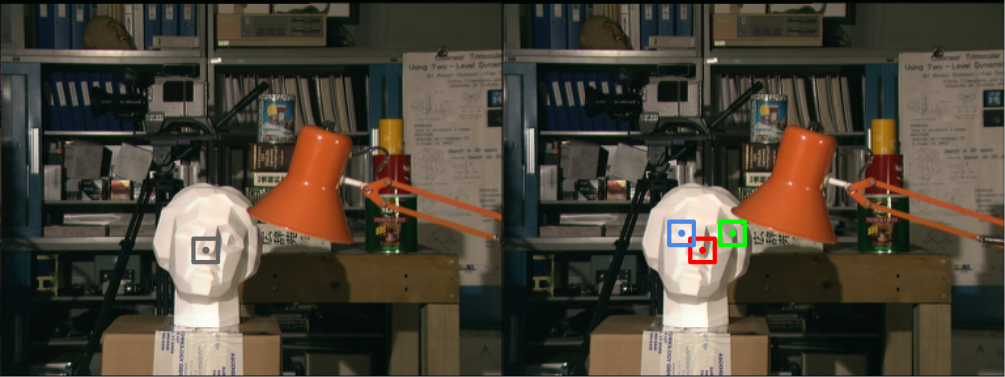
\includegraphics[height=0.40\textwidth]{fig/support_window}\\
\label{fig_support_window}
\caption{Support window to match (left) and the windows attempted/scanned on the other image (right).}
\end{center}
\end{figure}


%%%%%%%%%%%%%%%%%%%%%%%%%%%%%%%%%%%%%%%%%%%%%%%%%%%%%%%%%%%%%%%%%%%%%%

\subsubsection{Midterm presentation}
\begin{itemize}
	\item Did a presentation with the following information:
	\begin{itemize}
		\item Introduction.
		\item Challenges.
		\item Some theory.
		\item Tables and diagrams providing a picture of the work being done.
		\item Conclusions (so far).
	\end{itemize}
	\item The presentation can be found \href{https://docs.google.com/presentation/d/1_rqsAgTJxvEJvtRudIc00ItqAo_ZehuIC6Ru60WV8h8/edit?usp=sharing}{at this link}.
\end{itemize}


\subsection{Results}

%%%%%%%%%%%%%%%%%%%%%%%%%%%%%%%%%%%%%%%%%%%%%%%%%%%%%%%%%%%%%%%%%%%%%%

\subsubsection{Stereo vision depth detection}
\begin{itemize}
	\item Completed communication with the GPU.
	\item Designed and implemented the rendering pipeline.
	\begin{itemize}
		\item The last shader (disparity map) was not finished.
	\end{itemize}
\end{itemize}

%%%%%%%%%%%%%%%%%%%%%%%%%%%%%%%%%%%%%%%%%%%%%%%%%%%%%%%%%%%%%%%%%%%%%%

\subsubsection{Midterm presentation}
\begin{itemize}
	\item The presentation can be found \href{https://docs.google.com/presentation/d/1_rqsAgTJxvEJvtRudIc00ItqAo_ZehuIC6Ru60WV8h8/edit?usp=sharing}{at this link}.
\end{itemize}

\subsection{Pending}

\begin{itemize}
	\item \textbf{Turn line detection onto lane detection:} Add appropiate discrimination rules to get the lane.
	\item \textbf{Disparity map shader programming.}
	\item \textbf{Mechanical camera mount.}
\end{itemize}

\clearpage

%%%%%%%%%%%%%%%%%%%%%%%%%%%%%%%%%%%%%%%%%%%%%%%%

\fromto{Jun 30 - Jul 04}
\section{MEMORANDUM 10}

\subsection{Activities}

%%%%%%%%%%%%%%%%%%%%%%%%%%%%%%%%%%%%%%%%%%%%%%%%%%%%%%%%%%%%%%%%%%%%%%

\subsubsection{GPU shaders}
\begin{itemize}
	\item Decoding shader was written.
	\begin{itemize}
		\item This is to visually see the encoded data.
		\item Encoded data does not make a lot of sense visually.
	\end{itemize}
	\item Disparity map shader was written.
	\begin{itemize}
		\item Results are not as good as they can be.
		\item A different approach is being written.
		\begin{itemize}
			\item Current approach allows to check only for 11 levels of disparities.
			\item A more flexible and complex shader/pipeline is being written.
			\item It is needed specially because the distance between cameras has not been decided yet.
		\end{itemize}
	\end{itemize}
\end{itemize}

%%%%%%%%%%%%%%%%%%%%%%%%%%%%%%%%%%%%%%%%%%%%%%%%%%%%%%%%%%%%%%%%%%%%%%

\subsubsection{Integration of both cameras}
\begin{itemize}
	\item \textbf{Rewired.}
	\begin{itemize}
		\item Both cameras are clocked from the board with the STM32F429ZIT6.
		\item Both cameras' PWDN pins are connected to the same STM32F429ZIT6 pin (previously connected to ground).
		\item Remaining pins were connected to their respective microcontroller's board.
	\end{itemize}
	\item \textbf{Sofware related-work.}
	\begin{itemize}
		\item Synchronization logic was added.
		\begin{itemize}
			\item On both ends (STM32 and Raspberry).
		\end{itemize}
		\item It is very important to get both images at the same time.
		\item PWDN pin is used to:
		\begin{itemize}
			\item Halt internal device clock.
			\item Reset all internal counters.
			\item Keep registers.
		\end{itemize}
	\end{itemize}
\end{itemize}

%%%%%%%%%%%%%%%%%%%%%%%%%%%%%%%%%%%%%%%%%%%%%%%%%%%%%%%%%%%%%%%%%%%%%%

\subsubsection{Port to STM32F407VGT6's board.}
\begin{itemize}
	\item I am temporally going to work on this board too and the code had to be ported.
	\item SPI, DCMI, DMA and EXTI are now working on the other board too.
	\item Every pin had to be remapped.
	\item Register names were adjusted (cost of not using peripheral libraries).
	\item This board does not have external SDRAM.
	\item This microcontroller's maximum SPI speed is 42 MHz.
\end{itemize}

%%%%%%%%%%%%%%%%%%%%%%%%%%%%%%%%%%%%%%%%%%%%%%%%%%%%%%%%%%%%%%%%%%%%%%

\subsubsection{Threaded programming}
\begin{itemize}
	\item Threaded programming was needed because reading the frames from the camera requires very little processing power.
	\begin{itemize}
		\item Just waiting for the STM32 is underusing Raspberry resources.
	\end{itemize}
	\item POSIX threads were chosen for the task.
	\item Using real-time linux scheduling policies.
	\item The skeleton code is done.
	\item Tuning needs to be done when everything is ready.
	\item Only three threads are used at the moment.
	\begin{itemize}
		\item \textbf{Capture:} Reads frames from the camera to memory from the SPI peripheral. Signals the STM32 boards to keep the synchronization.
		\item \textbf{Depth:} Commands the GPU to perform the multiple rendering stages and get the resulting disparity map back to CPU memory.
		\item \textbf{Lane:} Executes the Hough Transform.
	\end{itemize}
\end{itemize}

\subsection{Results}

%%%%%%%%%%%%%%%%%%%%%%%%%%%%%%%%%%%%%%%%%%%%%%%%%%%%%%%%%%%%%%%%%%%%%%

\subsubsection{GPU shaders}
\begin{itemize}
	\item Decoding shader was written.
	\item Disparity map shader was written. Results were not very accurate and a second approach is being developed.
\end{itemize}

%%%%%%%%%%%%%%%%%%%%%%%%%%%%%%%%%%%%%%%%%%%%%%%%%%%%%%%%%%%%%%%%%%%%%%

\subsubsection{Integration of both cameras}
\begin{itemize}
	\item Several actions performed to get the frames of the cameras at the same moment.
	\item Has not been tested, but seems to work out of observations of the debugger and oscilloscope.
\end{itemize}

%%%%%%%%%%%%%%%%%%%%%%%%%%%%%%%%%%%%%%%%%%%%%%%%%%%%%%%%%%%%%%%%%%%%%%

\subsubsection{Port to STM32F407VGT6's board.}
\begin{itemize}
	\item The project that has been used on the other discovery board was ported to this one.
	\item It is working with its limitations (no SDRAM, SPI is slower).
\end{itemize}

%%%%%%%%%%%%%%%%%%%%%%%%%%%%%%%%%%%%%%%%%%%%%%%%%%%%%%%%%%%%%%%%%%%%%%

\subsubsection{Threaded programming}
\begin{itemize}
	\item Skeleton project is ready, using real-time linux scheduling policies.
	\item Multithread program consisting of three threads:
	\begin{itemize}
		\item Capture.
		\item Depth.
		\item Lane.
	\end{itemize}
\end{itemize}

\subsection{Pending}

\begin{itemize}
	\item Camera mount mechanism.
	\item New disparity map shader.
	\item Integration into the multithreaded program.
\end{itemize}

\clearpage

%%%%%%%%%%%%%%%%%%%%%%%%%%%%%%%%%%%%%%%%%%%%%%%%

\fromto{Jul 07 - Aug 01}
\section{MEMORANDUM 11}

\subsection{Activities}
%%%%%%%%%%%%%%%%%%%%%%%%%%%%%%%%%%%%%%%%%%%%%%%%%%%%%%%%%%%%%%%%%%%%%%

\subsubsection{Refinements to the threaded code}
\begin{itemize}
	\item Scheduling policies for POSIX threads were studied in more detail and some portions of the code were fixed.
	\item Added command line interface to the program to set these options.
	\item This code has not been tested yet.
\end{itemize}

%%%%%%%%%%%%%%%%%%%%%%%%%%%%%%%%%%%%%%%%%%%%%%%%%%%%%%%%%%%%%%%%%%%%%%

\subsubsection{Compatible WebGL platform}
As stated earlier in this report WebGL is based on OpenGL ES 2.0--which is the OpenGL implementation found in the Raspberry. A WebGL platform/codebase was developed to take advantage of the following benefits:
\begin{itemize}
	\item Faster validation of shader programs.
	\item Easier to share/show results (most people have access to a WebGL compatible browser and internet).
	\item Better evaluation tools (browsers have built in tools to profile GPU activity).
	\item Portability (few to no changes are needed to run the same code on the Raspberry GPU).
\end{itemize}

Tasks performed include:
\begin{itemize}
	\item Porting the C code to javascript.
	\item Setting up a web server.
	\item Coding an interface to the code through HTTP requests.
\end{itemize}

%%%%%%%%%%%%%%%%%%%%%%%%%%%%%%%%%%%%%%%%%%%%%%%%%%%%%%%%%%%%%%%%%%%%%%
\subsubsection{Modifications to the codebase}

During the development of the WebGL platform several modifications were done to the code that commands the GPU. The objectives were to improve:
\begin{itemize}
	\item Performance.
	\begin{itemize}
		\item Initialize uniforms outside the drawing functions.
		\item Only change programs if necessary.
		\item Only set buffers once.
		\item Everything that could be done outside function calls is done outside function calls.
	\end{itemize}
	\item Flexibility.
	\begin{itemize}
		\item Different stereo-matching methods can be added without modifying the core of the code.
	\end{itemize}
	\item Portability.
	\begin{itemize}
		\item Code on the Raspberry should mimic the WebGL platform.
		\item Language is different but logic is the same.
		\item GPU shader programs are exactly the same.
	\end{itemize}
\end{itemize}

%%%%%%%%%%%%%%%%%%%%%%%%%%%%%%%%%%%%%%%%%%%%%%%%%%%%%%%%%%%%%%%%%%%%%%
\subsubsection{Documentation/presentation}
Figures (\ref{fig_hwconnectionsglobal}, \ref{fig_both_frames}, \ref{fig_matching1-result}) and tables (\ref{tab_boardpins_final}) were generated.

These figures show the hardware connections for both boards, their signaling and the output from the GPU stereo match, respectively.

The table shows the signals and the corresponding pins from each STM32 board and the Rasberry.

\begin{figure}[ht!]
\begin{center}
\includegraphics[height=0.50\textwidth]{fig/hwconnectionsglobal}\\
\caption{Signals connected between the OV7670s, STM32s and the Raspberry Pi.}
\label{fig_hwconnectionsglobal}
\end{center}
\end{figure}

\begin{table}[ht!]
\begin{center}
\begin{tabular}{| c | c | c | c | c |}
\hline
Signal	& Peripheral	& Pin left	& Pin right	& Pin Raspberry \\
\hline
D0	& \multirow{11}{*} {DCMI} & PA09 & PC06 & - \\
D1	& & PA10 & PC07 & - \\
D2	& & PC08 & PC08 & - \\
D3	& & PG11 & PC09 & - \\
D4	& & PE04 & PE04 & - \\
D5	& & PD03 & PB06 & - \\
D6	& & PE05 & PE05 & - \\
D7	& & PE06 & PE06 & - \\
HSYNC	& & PA04 & PA04 & - \\
PXCLK	& & PA06 & PA06 & - \\
VSYNC	& & PB07 & PB07 & - \\ \hline
CS*	& \multirow{2}{*}{EXTI} & PC03 \& PD04 & PD03 \& PC04 & P13(L) / P15(R) \\ 
FS**	& & PG02 & PA01 & P11 \\ \hline
MISO**	& \multirow{2}{*}{SPI} & PF08 & PB04 & P21 \\
SCK**	& & PF07 & PA05 & P23 \\ \hline
SDIO\_C & \multirow{7}{*}{GPIO} & PC11 & PD10 & - \\
SDIO\_D & & PC12 & PD11 & - \\
CS Gyro & & PC01 & - & - \\
CS LCD	& & PC02 & - & - \\
EN LCD	& & PF10 & - & - \\
PWDN	& & PC13 & - & - \\
CS LIS3 & & - & PE03 & - \\ \hline
MCO2	& MCO & PC09 & - & - \\
\hline
\end{tabular}
\caption[Final selections of pins.]{Final selections of pins for both boards to be used by the application.}
\label{tab_boardpins_final}
\end{center}
\end{table}

\begin{figure}[t]
\begin{center}
\scalebox{1}{
\begin{tikztimingtable}
	FS			& H H 38{L} H H\\
	CSL			& H H 14{L} ;[dotted] 2{L}; 3{L} 19{H} H H \\
	CSR			& H H 19{H} 14{L} ;[dotted] 2{L}; 3{L} H H \\
	CLK			& L L L 13{C} ;[dotted] 2{C}; 3{C} L 13{C} ;[dotted] 2{C}; 3{C} L L \\
	MISO			& U U U 18D{Left image pixel data} U 18D{Right image pixel data} U U\\
\end{tikztimingtable}
}
\caption{Time diagram showing the communication protocol between the Raspberry and both STM32 microcontrollers.}
\label{fig_both_frames}
\end{center}
\end{figure}

\begin{figure}[ht!]
\begin{center}
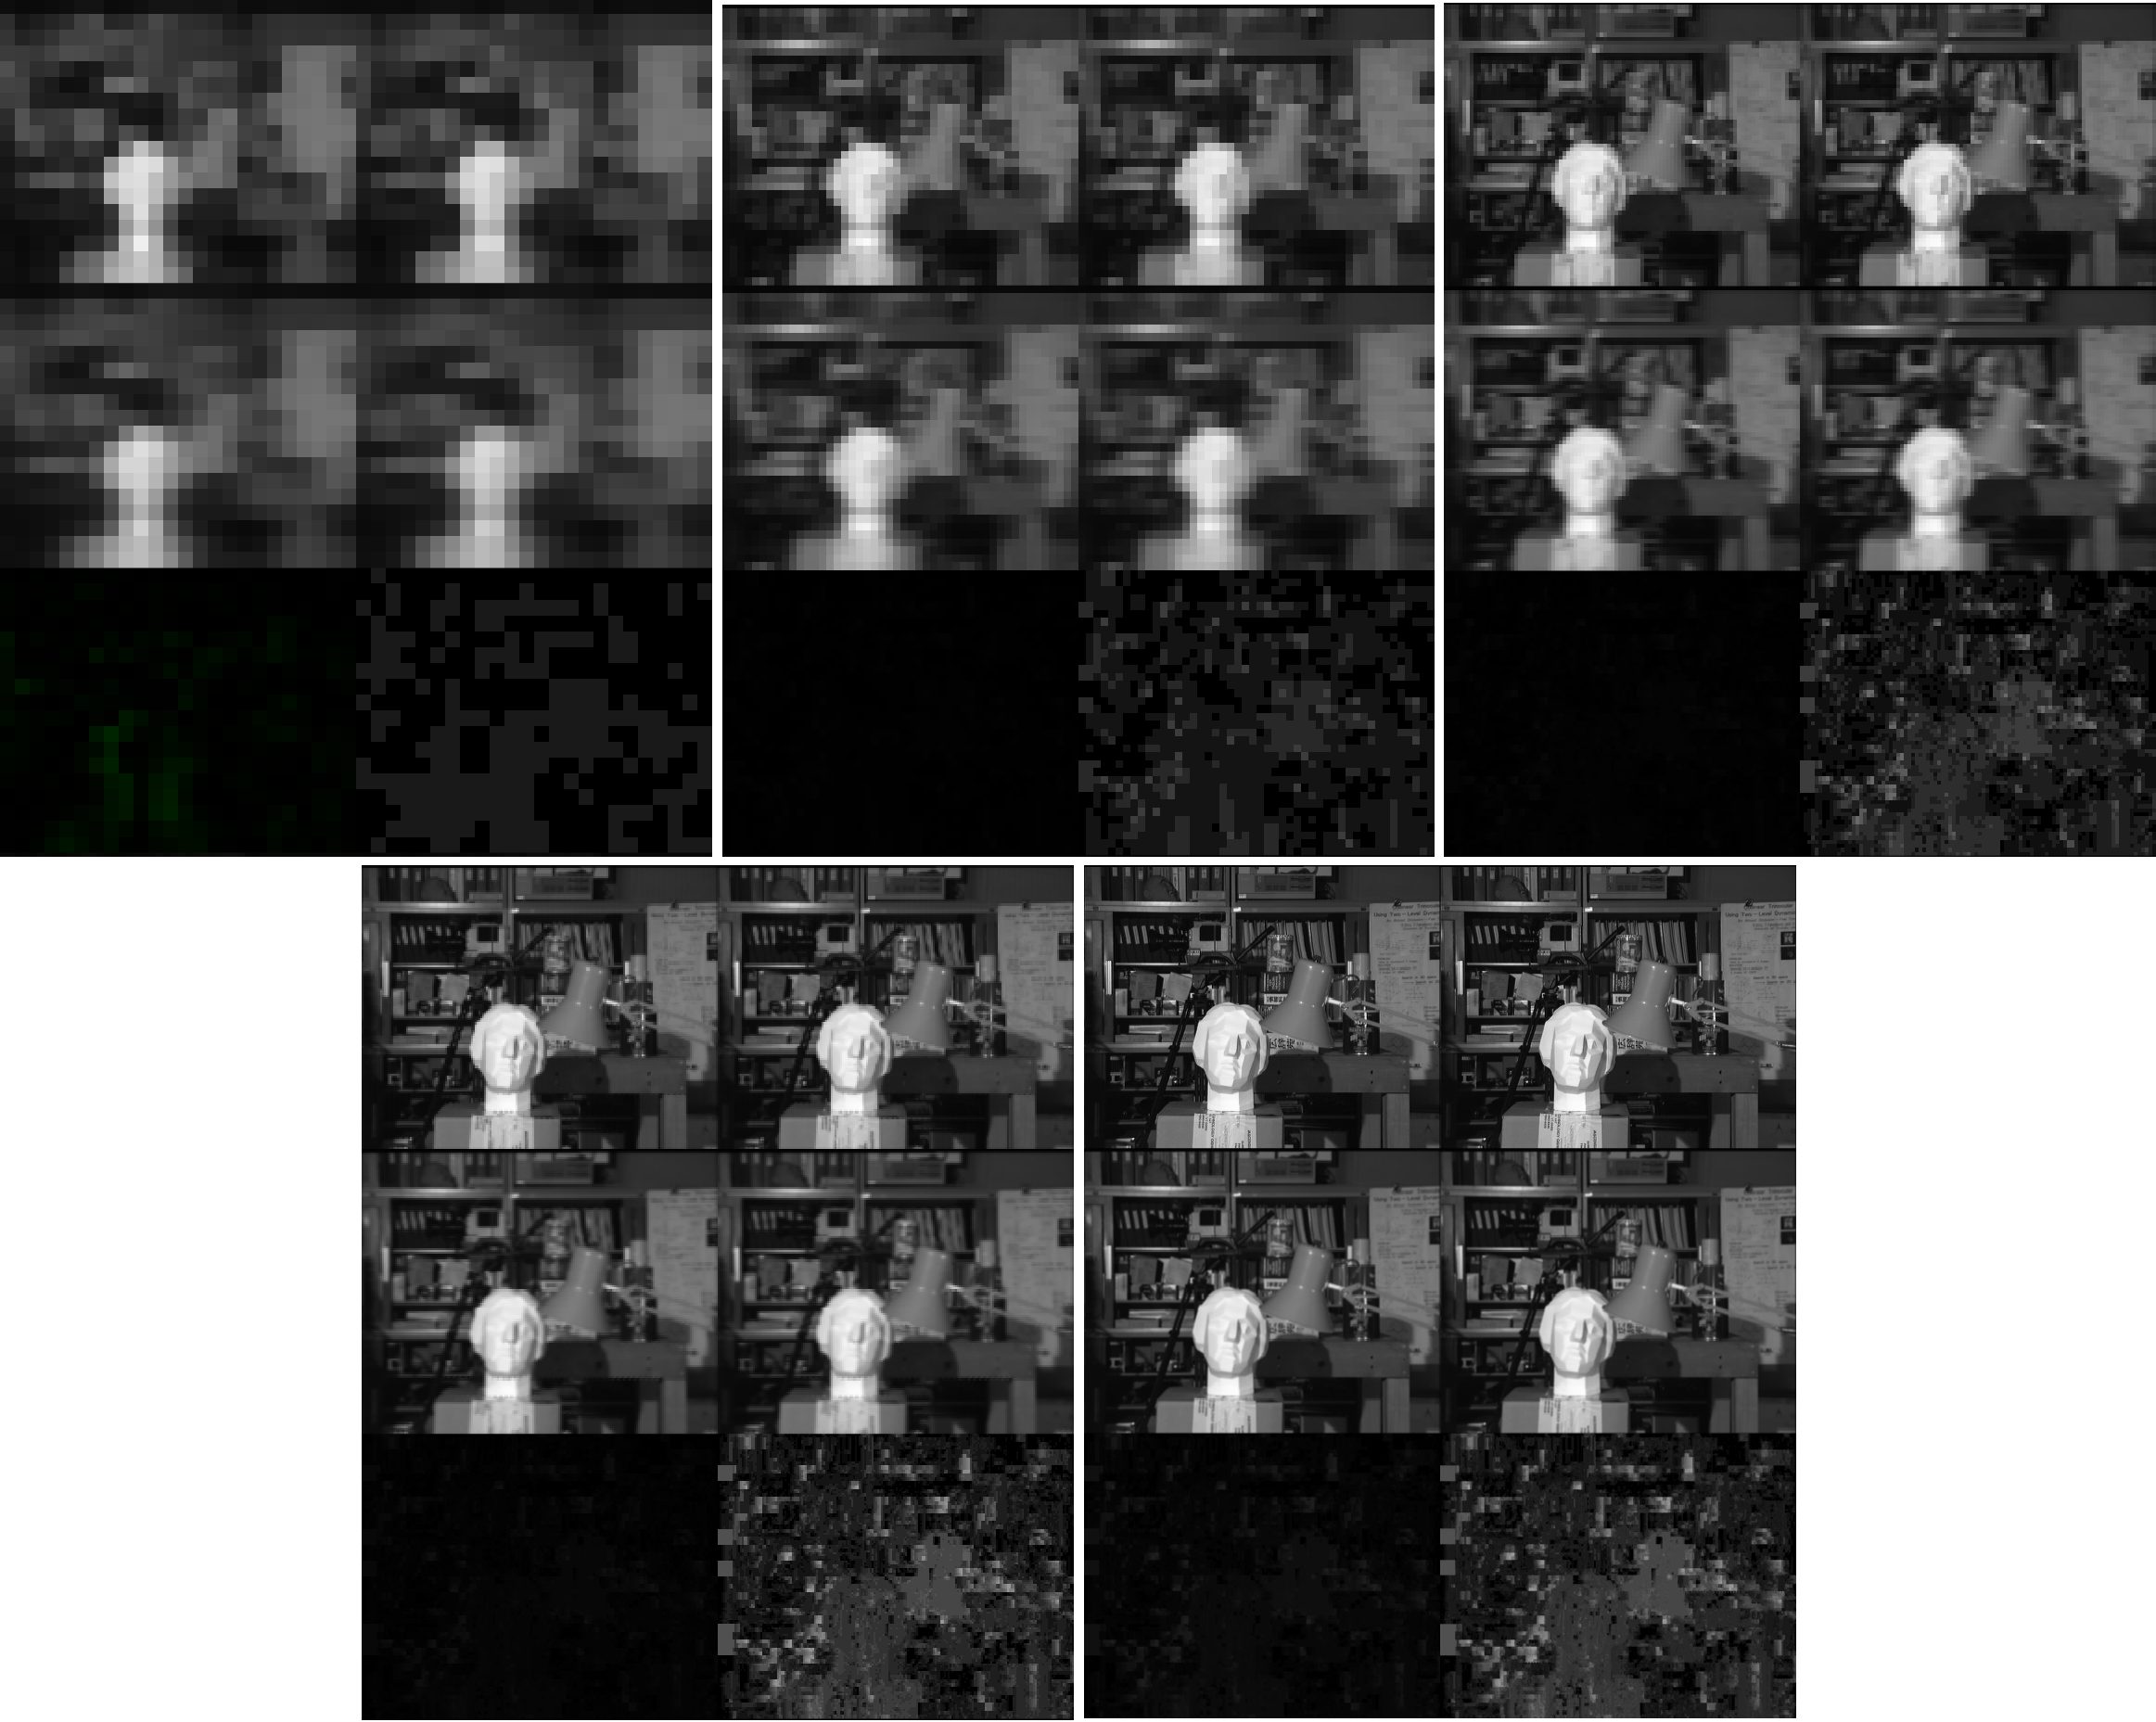
\includegraphics[width=12cm]{fig/matching1-result}\\
\caption{Tsukuba images matched on the GPU, image taken from the WebGL platform.}
\label{fig_matching1-result}
\end{center}
\end{figure}


%%%%%%%%%%%%%%%%%%%%%%%%%%%%%%%%%%%%%%%%%%%%%%%%%%%%%%%%%%%%%%%%%%%%%%
\subsubsection{Stereo-matching on GPU}
\begin{itemize}
	\item A method has been fully implemented in GPU.
	\item Results from this method are shown in figure \ref{fig/matching1-result.tex}.
\end{itemize}

%%%%%%%%%%%%%%%%%%%%%%%%%%%%%%%%%%%%%%%%%%%%%%%%%%%%%%%%%%%%%%%%%%%%%%
\subsubsection{Paper}

I am writing a paper in which I will discuss and conclude about:
\begin{itemize}
	\item GPGPU in general.
	\item GPGPU on embedded GPUs (in general and specifically through OpenGL ES 2.0).
	\item Solving the stereo matching problem on the GPU.
	\item The specifics of doing this on the Raspberry (which is a common board, but will mention other options in general).
	\item Report the results (time, accuracy) of a case study.
	\item Share code and results through the WebGL platform.
\end{itemize}

\subsection{Results}

%%%%%%%%%%%%%%%%%%%%%%%%%%%%%%%%%%%%%%%%%%%%%%%%%%%%%%%%%%%%%%%%%%%%%%
\subsubsection{Refinements to the threaded code}
\begin{itemize}
	\item Interface to the parameters that would affect the real time Linux scheduling policies.
	\item Fixed some errors.
\end{itemize}
%%%%%%%%%%%%%%%%%%%%%%%%%%%%%%%%%%%%%%%%%%%%%%%%%%%%%%%%%%%%%%%%%%%%%%
\subsubsection{Compatible WebGL platform}
\begin{itemize}
	\item Fully compatible with the Raspberry WebGL platform to develop GPU code.
\end{itemize}
%%%%%%%%%%%%%%%%%%%%%%%%%%%%%%%%%%%%%%%%%%%%%%%%%%%%%%%%%%%%%%%%%%%%%%
\subsubsection{Modifications to the codebase}
\begin{itemize}
	\item Code was modified to improve performance, flexibility and portability.
\end{itemize}
%%%%%%%%%%%%%%%%%%%%%%%%%%%%%%%%%%%%%%%%%%%%%%%%%%%%%%%%%%%%%%%%%%%%%%
\subsubsection{Documentation/presentation}
\begin{itemize}
	\item Tables and figures were done for documentation/presentation purposes.
\end{itemize}
%%%%%%%%%%%%%%%%%%%%%%%%%%%%%%%%%%%%%%%%%%%%%%%%%%%%%%%%%%%%%%%%%%%%%%
\subsubsection{Stereo-matching on GPU}
\begin{itemize}
	\item A method for stereo-matching was implemented through OpenGL shaders.
\end{itemize}
%%%%%%%%%%%%%%%%%%%%%%%%%%%%%%%%%%%%%%%%%%%%%%%%%%%%%%%%%%%%%%%%%%%%%%
\subsubsection{Paper}
\begin{itemize}
	\item A paper is being written.
\end{itemize}



\clearpage

%%%%%%%%%%%%%%%%%%%%%%%%%%%%%%%%%%%%%%%%%%%%%%%%

\section{APPENDIX}
\subsection{Gantt A}
\begin{figure}[ht!]
\begin{center}
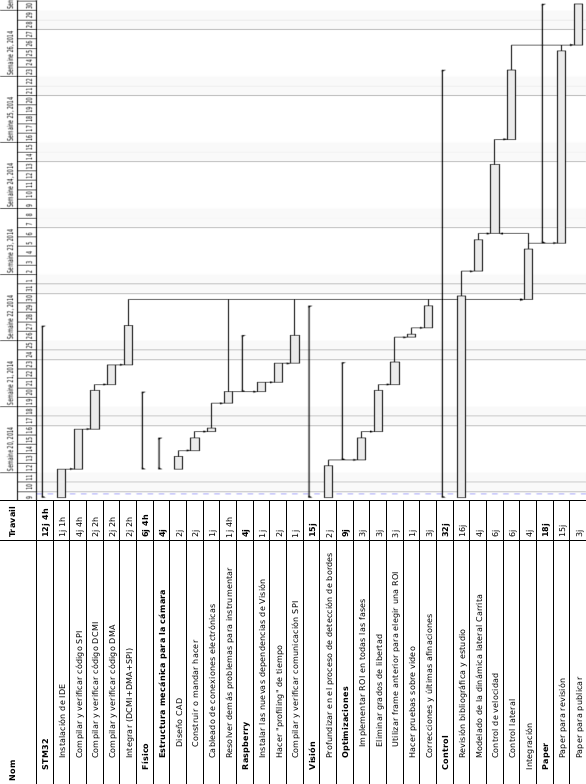
\includegraphics[height=1.3\textwidth]{fig/ganttscaled}\\
\caption{Gantt chart for the first two months.}
\label{fig_ganttA}
\end{center}
\end{figure}

\subsection{Camera mount mechanism drawings}
\begin{figure}[ht!]
\begin{center}
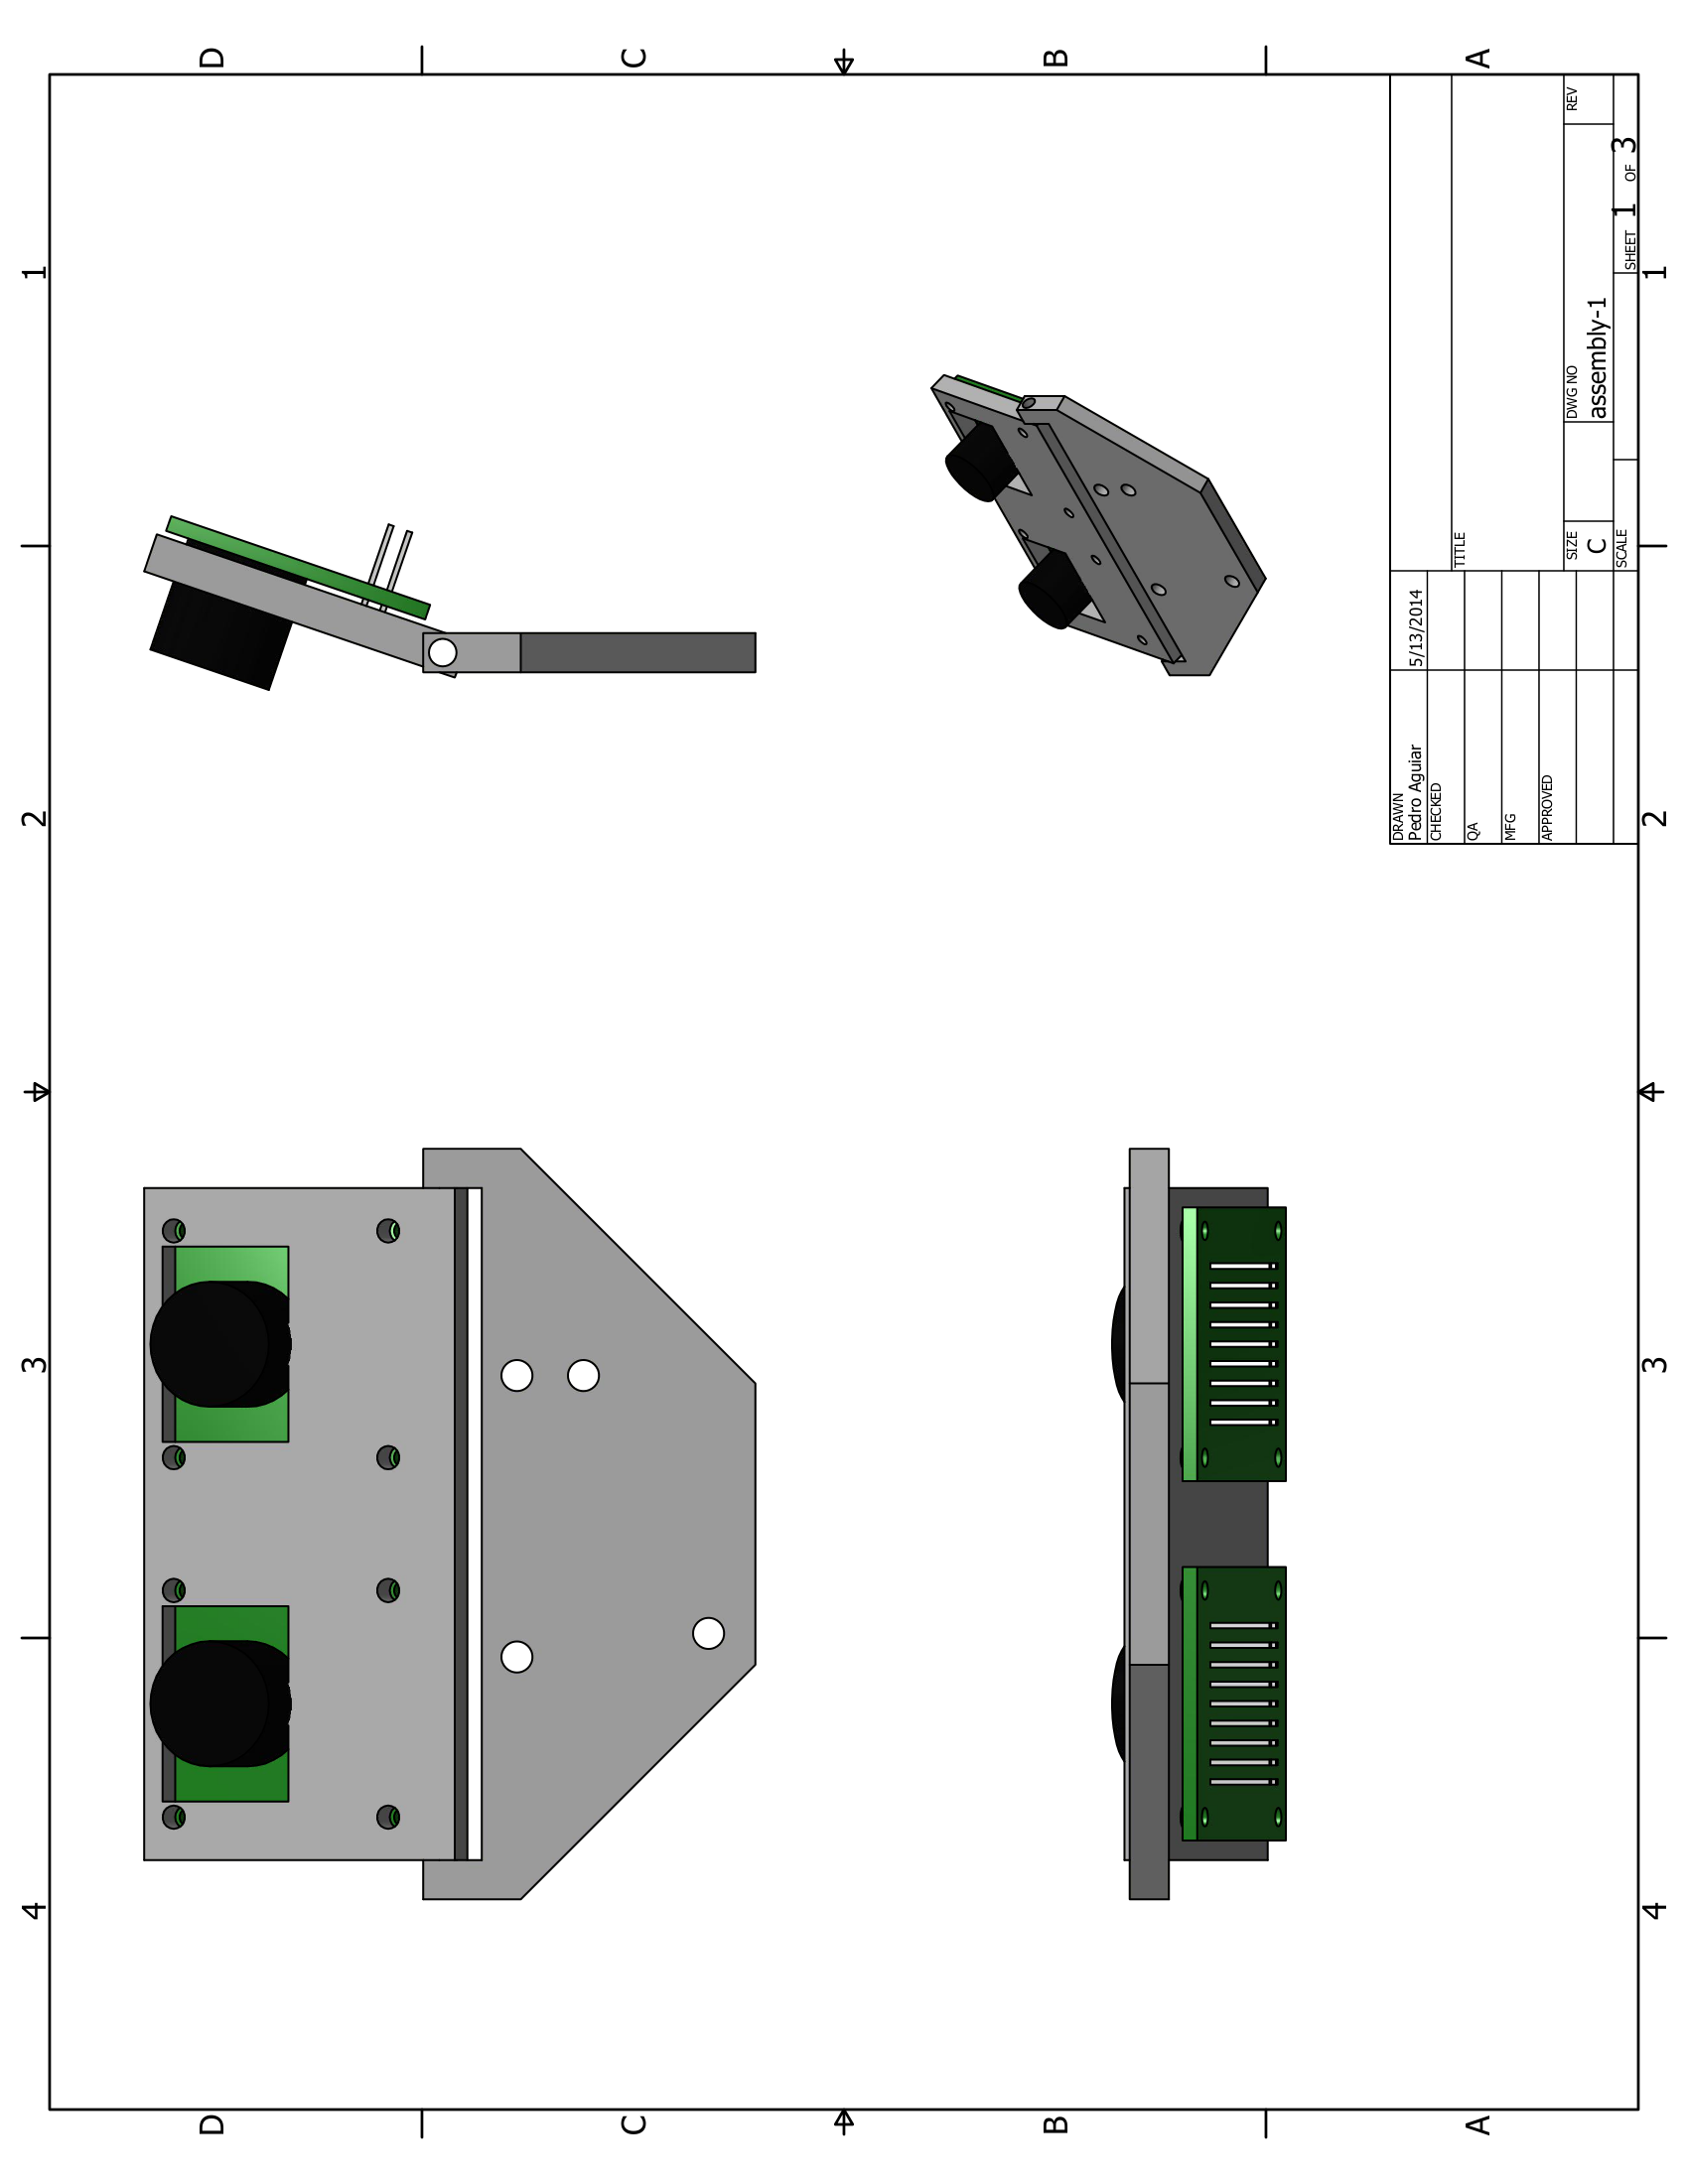
\includegraphics[height=1.2\textwidth]{fig/cammountp1}\\
\caption[Drawing. Assembled camera mount.]{Camera mount mechanism drawings: Assembled camera mount.}
\label{fig_cammountp1}
\end{center}
\end{figure}

\begin{figure}[ht!]
\begin{center}
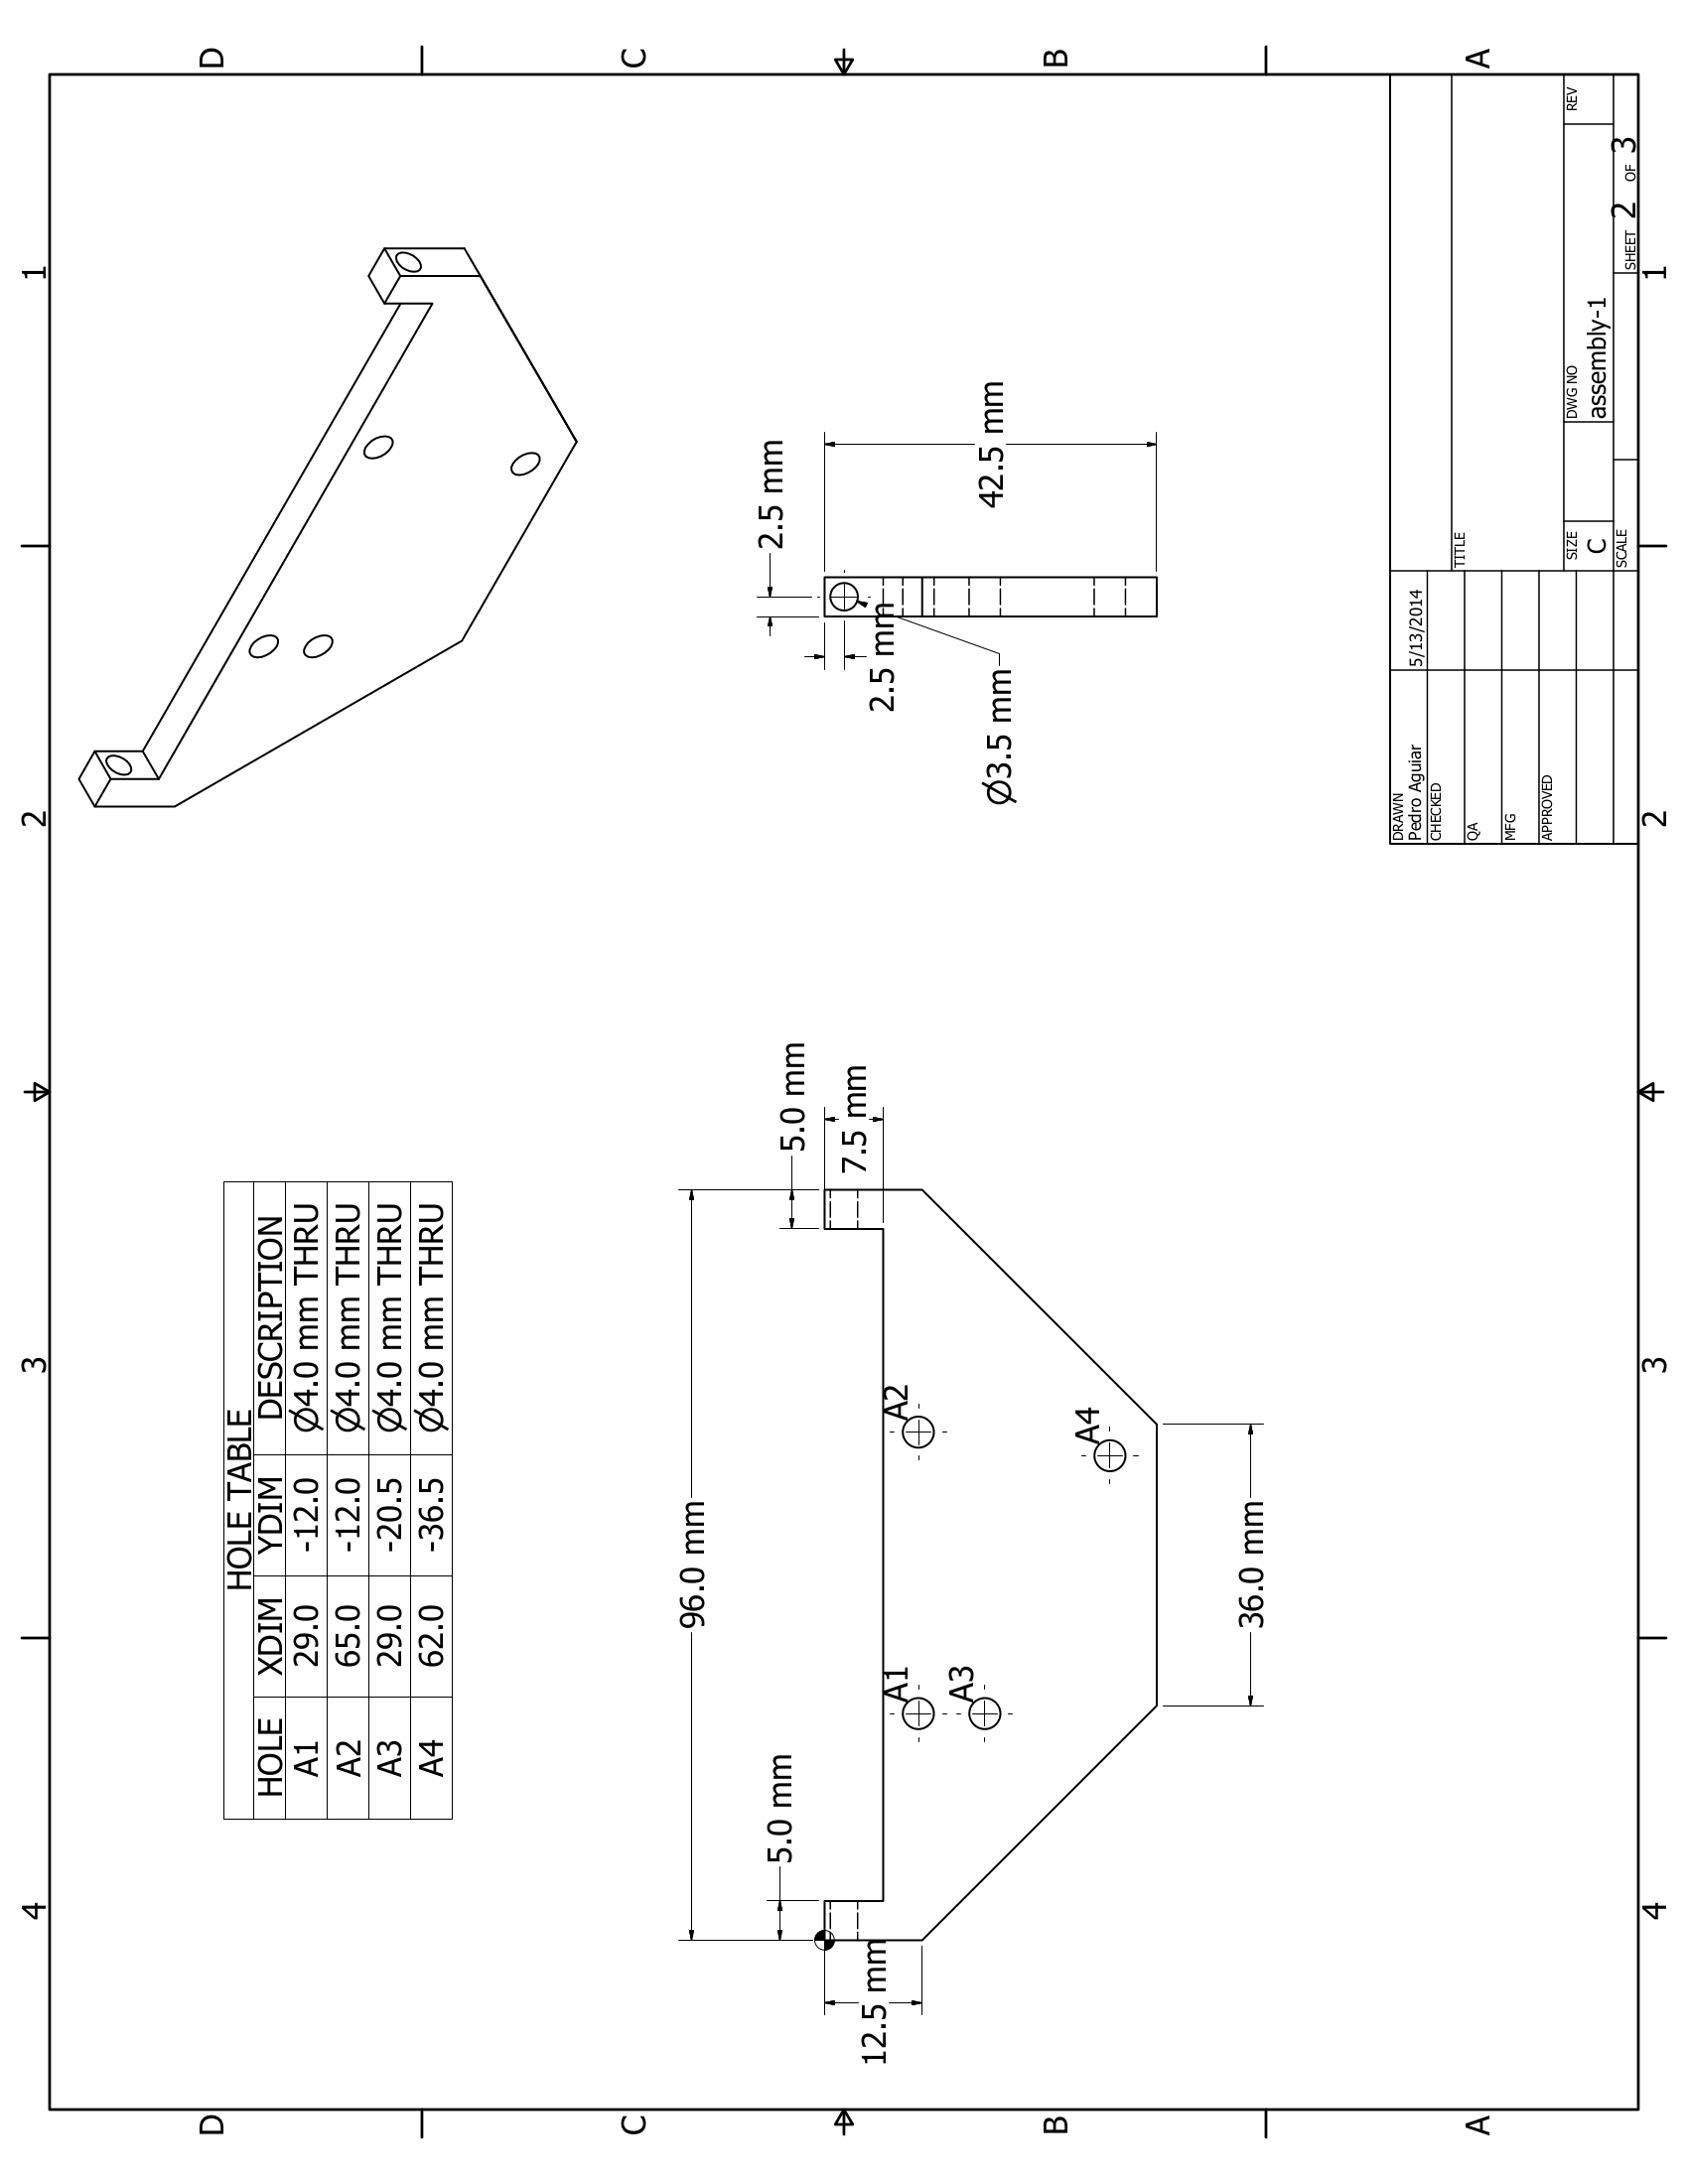
\includegraphics[height=1.2\textwidth]{fig/cammountp2}\\
\caption[Drawing. Camera part.]{Camera mount mechanism drawings: camera part.}
\label{fig_cammountp2}
\end{center}
\end{figure}

\begin{figure}[ht!]
\begin{center}
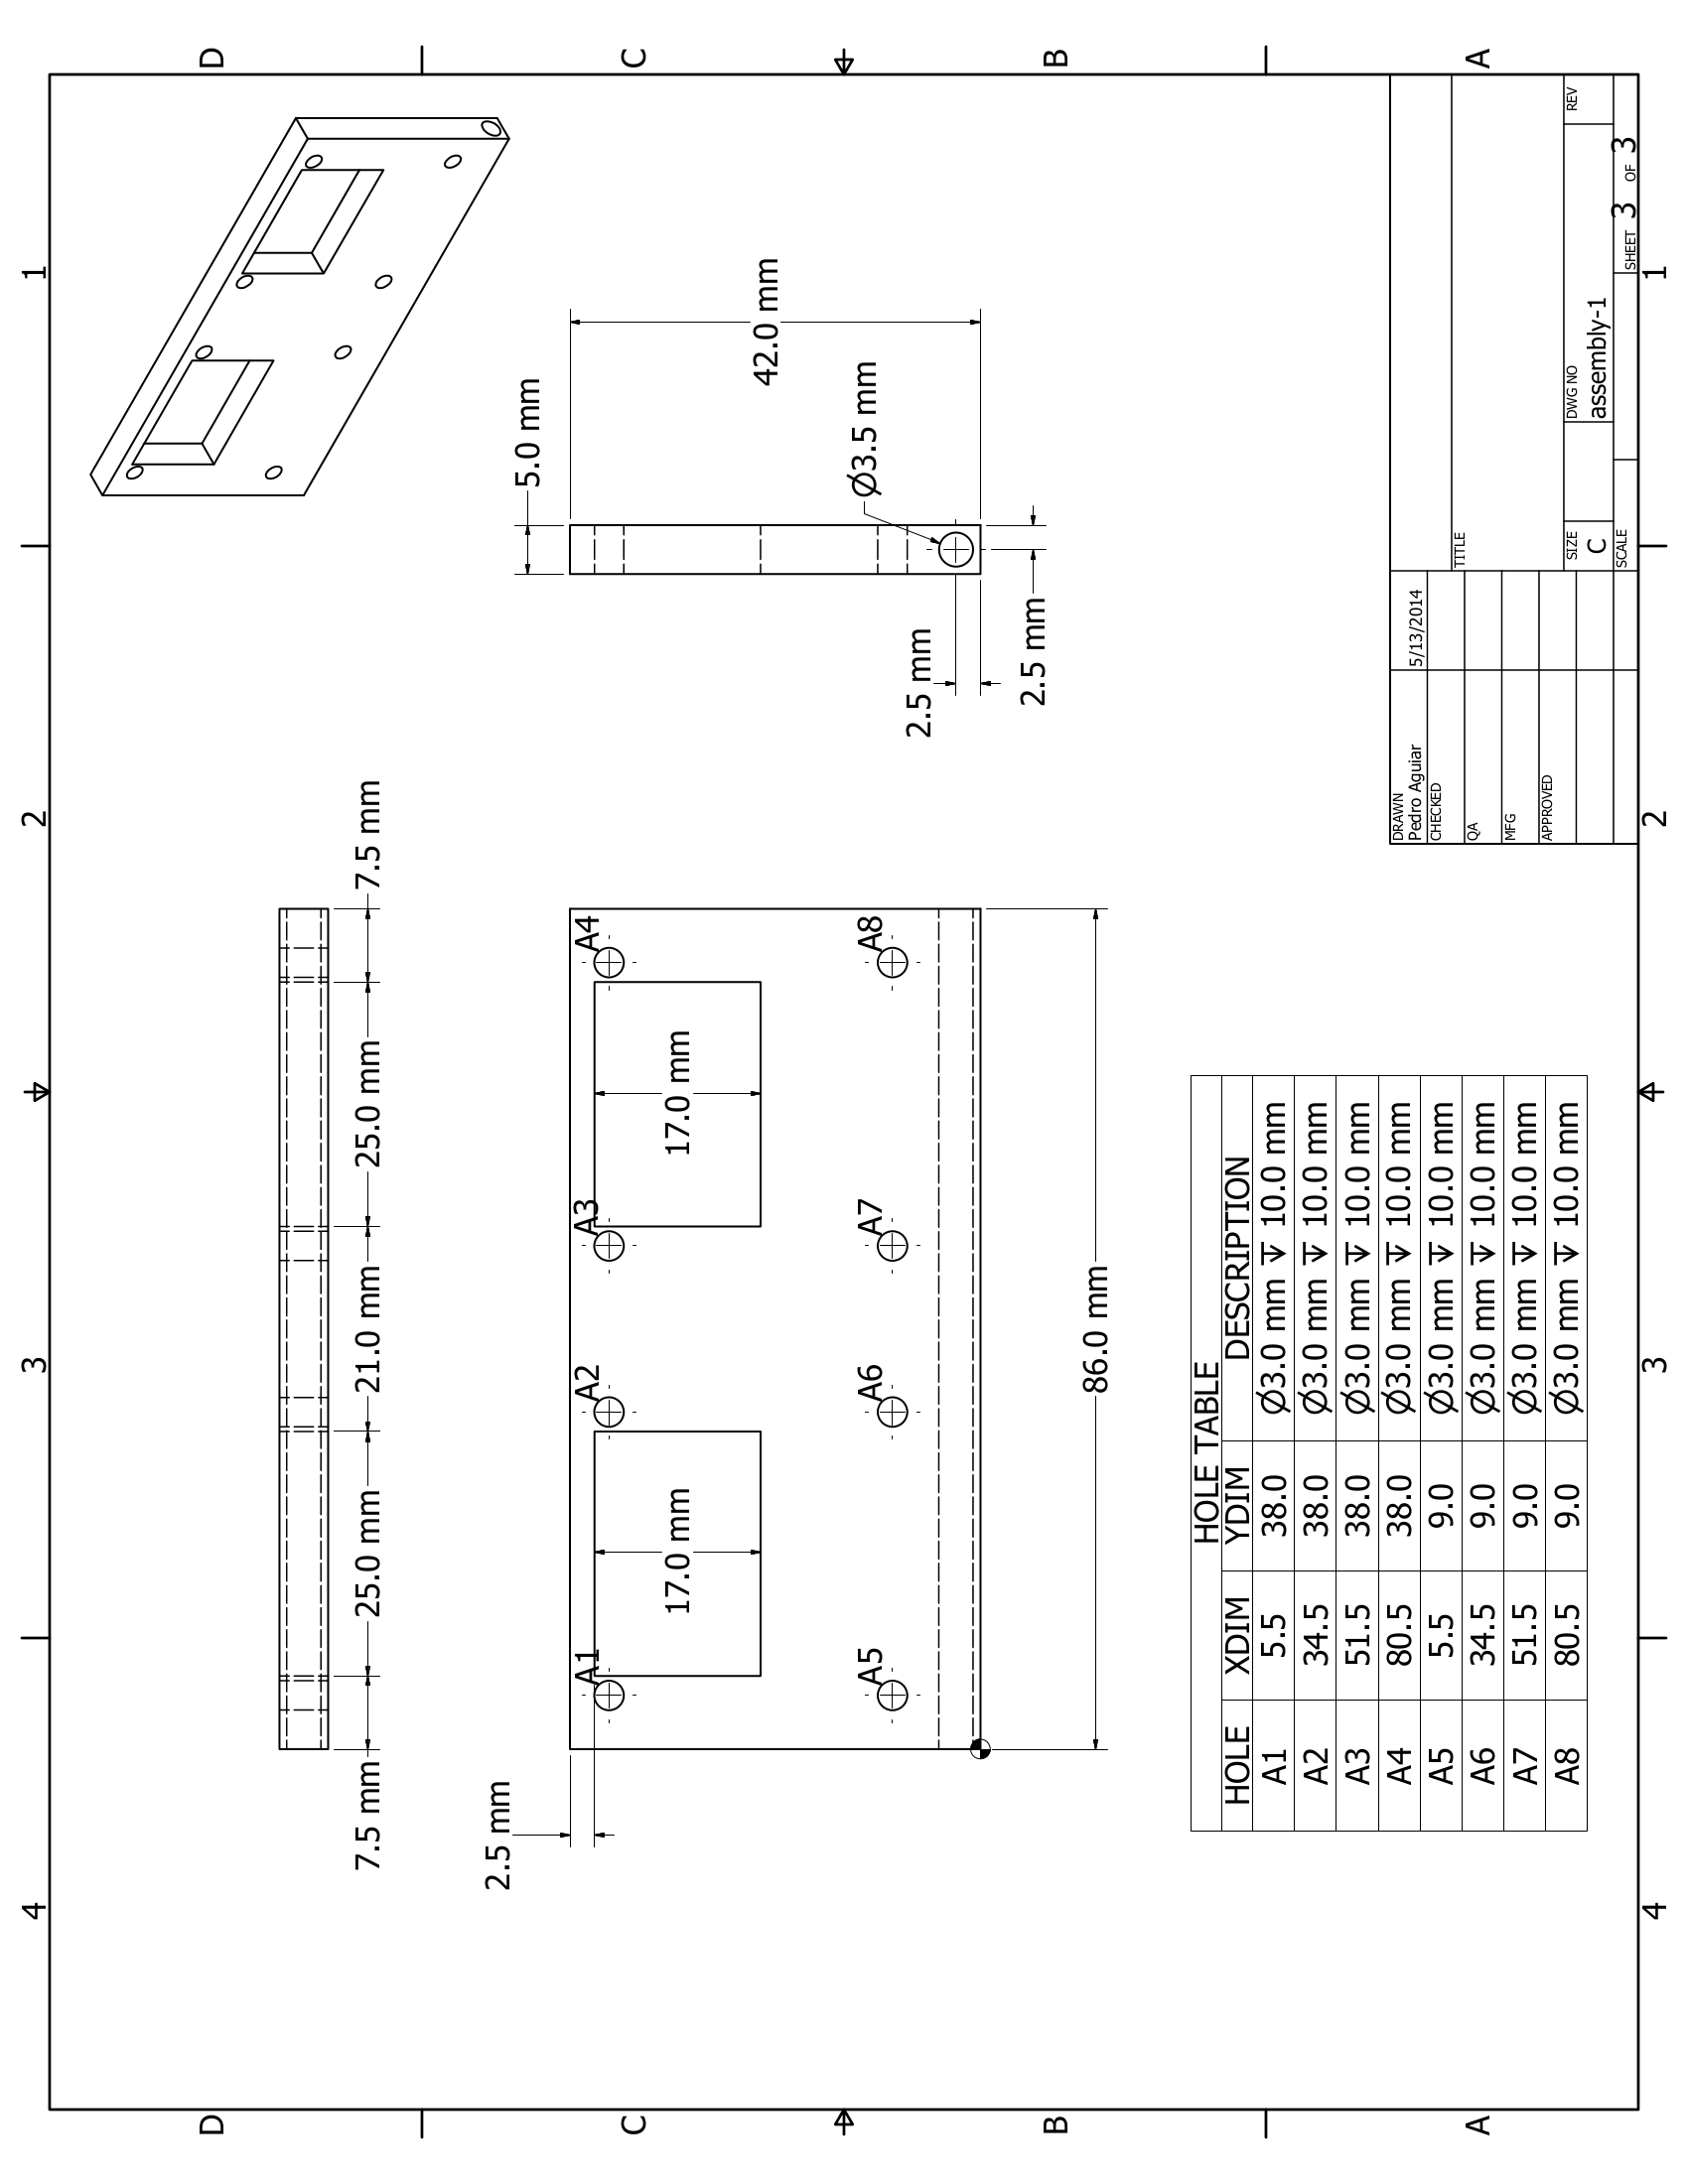
\includegraphics[height=1.2\textwidth]{fig/cammountp3}\\
\caption[Drawing. Carrita's part.]{Camera mount mechanism drawings: Carrita's part.}
\label{fig_cammountp3}
\end{center}
\end{figure}

\clearpage

\begin{thebibliography}{9}
 \bibitem{cummings}
	Chris Cummings,
	\emph{Gpu accelerated image processing on raspberry pi}. http://youtu.be/yQZISXIFjaQ

 \bibitem{dubska}
	Markéta Dubská, Adam Herout,
	\emph{Real-Time Detection of Lines using Parallel Coordinates and OpenGL}. 

\end{thebibliography}

\end{document}
